%% ============================================================
%%  LAPORAN PROGRESS TUGAS AKHIR
%%  Electronic Nose: CSV Profiler, OTA Server & Simulasi ESP32
%%  Compile: pdflatex -shell-escape laporan_progress.tex
%% ============================================================
\documentclass[12pt,a4paper]{report}

% ─── PACKAGE ────────────────────────────────────────────────
\usepackage[T1]{fontenc}
\usepackage[utf8]{inputenc}
\usepackage[indonesian]{babel}
\usepackage{geometry}
\usepackage{graphicx}
\usepackage{float}
\usepackage{caption}
\usepackage{subcaption}
\usepackage{booktabs}
\usepackage{array}
\usepackage{tabularx}
\usepackage{longtable}
\usepackage{listings}
\usepackage{xcolor}
\usepackage{hyperref}
\usepackage{fancyhdr}
\usepackage{titlesec}
\usepackage{enumitem}
\usepackage{amsmath}
\usepackage{parskip}
\usepackage{tcolorbox}
\usepackage{lmodern}

% ─── GEOMETRY ────────────────────────────────────────────────
\geometry{
  a4paper,
  top=3cm, bottom=3cm,
  left=3.5cm, right=2.5cm,
  headheight=15pt
}

% ─── WARNA ──────────────────────────────────────────────────
\definecolor{darkblue}{RGB}{0,51,102}
\definecolor{codeblue}{RGB}{0,0,180}
\definecolor{codegray}{RGB}{128,128,128}
\definecolor{codegreen}{RGB}{0,128,0}
\definecolor{codepurple}{RGB}{148,0,211}
\definecolor{backcolor}{RGB}{245,245,245}
\definecolor{accentblue}{RGB}{0,102,204}
\definecolor{noteboxbg}{RGB}{230,240,255}
\definecolor{noteboxborder}{RGB}{0,102,204}

% ─── HEADER/FOOTER ──────────────────────────────────────────
\pagestyle{fancy}
\fancyhf{}
\fancyhead[L]{\small\textit{Laporan Progress Tugas Akhir --- Electronic Nose}}
\fancyhead[R]{\small\textit{\thepage}}
\fancyfoot[C]{\small\textit{Dokumen untuk keperluan akademis}}
\renewcommand{\headrulewidth}{0.4pt}
\renewcommand{\footrulewidth}{0.4pt}

% ─── CHAPTER TITLE STYLE ───────────────────────────────────
\titleformat{\chapter}[block]
  {\normalfont\LARGE\bfseries\color{darkblue}\raggedright}
  {\thechapter.}{0.8em}{}
\titlespacing*{\chapter}{0pt}{-10pt}{20pt}

% ─── CODE LISTING STYLE ─────────────────────────────────────
\lstdefinestyle{pythonstyle}{
  backgroundcolor=\color{backcolor},
  commentstyle=\color{codegreen},
  keywordstyle=\color{codeblue}\bfseries,
  numberstyle=\tiny\color{codegray},
  stringstyle=\color{codepurple},
  basicstyle=\ttfamily\footnotesize,
  breakatwhitespace=false,
  breaklines=true,
  captionpos=b,
  keepspaces=true,
  numbers=left,
  numbersep=8pt,
  showspaces=false,
  showstringspaces=false,
  showtabs=false,
  tabsize=4,
  frame=single,
  rulecolor=\color{darkblue!30},
  xleftmargin=12pt,
  xrightmargin=4pt
}
\lstset{style=pythonstyle}

% ─── INFO BOX ───────────────────────────────────────────────
\newenvironment{infobox}[1]{%
  \begin{tcolorbox}[
    colback=noteboxbg,
    colframe=noteboxborder,
    title={\textbf{#1}},
    fonttitle=\small\bfseries,
    boxrule=0.8pt,
    arc=4pt,
    left=6pt, right=6pt,
    top=4pt, bottom=4pt
  ]
}{%
  \end{tcolorbox}
}

% ─── HYPERREF SETUP ─────────────────────────────────────────
\hypersetup{
  colorlinks=true,
  linkcolor=darkblue,
  urlcolor=accentblue,
  citecolor=darkblue,
  pdftitle={Laporan Progress TA --- Electronic Nose},
  pdfauthor={Moreno Rizkihakiki, Muhammad Alif Al Ayyubi, Mochammad Ilham Fandy R., Gatam Arbi Muhammad},
  pdfsubject={Sistem Penciuman Elektronik (E-Nose) berbasis ESP32}
}

% ─── CAPTION STYLE ──────────────────────────────────────────
\captionsetup{
  font=small,
  labelfont={bf,color=darkblue},
  margin=10pt
}

\graphicspath{{./image/}}

%% ============================================================
%%  DOKUMEN MULAI
%% ============================================================
\begin{document}

% ─── HALAMAN JUDUL ──────────────────────────────────────────
\begin{titlepage}
  \thispagestyle{empty}
  \centering
  \vspace*{0.5cm}
  {\Large\bfseries\color{darkblue} LAPORAN PROGRESS TUGAS AKHIR\par}
  \vspace{0.3cm}
  {\color{darkblue}\rule{\linewidth}{1.5pt}}\par
  \vspace{0.8cm}
  {\LARGE\bfseries\color{darkblue}\linespread{1.25}\selectfont
    Perancangan Sistem Electronic Nose\\
    Berbasis ESP32-S3 dengan\\
    Infrastruktur CSV Profiler, OTA Update,\\
    dan Simulasi Telemetri ThingsBoard\par
  }
  \vspace{1.2cm}
  {\large\bfseries Disusun oleh:\par}
  \vspace{0.4cm}
  \begin{tabular}{rl}
    \textbf{Moreno Rizkihakiki}              & NRP. 2042241088 \\
    \textbf{Muhammad Alif Al Ayyubi}         & NRP. 2042241070 \\
    \textbf{Mochammad Ilham Fandy R.}        & NRP. 2042241107 \\
    \textbf{Gatam Arbi Muhammad}             & NRP. 2042241100 \\
  \end{tabular}
  \vfill
  {\large Departemen Teknik Instrumentasi\par}
  \vspace{0.15cm}
  {\large\bfseries Fakultas Vokasi\par}
  \vspace{0.15cm}
  {\large\bfseries Institut Teknologi Sepuluh Nopember\par}
  \vspace{0.15cm}
  {\large Surabaya\par}
  \vspace{0.6cm}
  {\large \today\par}
  \vspace*{0.3cm}
\end{titlepage}

% ─── DAFTAR ISI ─────────────────────────────────────────────
\pagenumbering{roman}
\tableofcontents
\newpage
\listoffigures
\newpage
\listoftables
\newpage
\pagenumbering{arabic}

%% ============================================================
\chapter{Pendahuluan}
%% ============================================================

\section{Latar Belakang}

Sistem penciuman elektronik (\textit{Electronic Nose} / E-Nose) merupakan instrumen
yang meniru kemampuan indera penciuman manusia menggunakan susunan sensor gas dan
algoritma pengenalan pola. Teknologi ini memiliki berbagai aplikasi, di antaranya
dalam bidang keamanan pangan, deteksi bahan berbahaya, diagnosa medis berbasis bau,
serta pemantauan kualitas udara.

Tugas Akhir ini merancang sebuah sistem E-Nose berbasis mikrokontroler
\textbf{ESP32-S3} yang mengintegrasikan delapan sensor gas (keluarga MQ dan TGS)
bersama sensor lingkungan DHT22. Agar pengembangan dapat berlangsung efisien dan
terukur, sistem dilengkapi dengan:

\begin{itemize}[leftmargin=2cm, itemsep=2pt]
  \item \textbf{CSV Data Profiler} --- \textit{dashboard} berbasis web untuk
        analisis eksploratori data (EDA) sensor secara otomatis;
  \item \textbf{OTA (\textit{Over-The-Air}) Firmware Server} --- infrastruktur
        pembaruan \textit{firmware} ESP32 secara nirkabel;
  \item \textbf{Simulasi Telemetri} --- firmware Rust (ESP32-S3) yang menghasilkan data
        sensor sintetik realistis untuk memvalidasi seluruh alur pengiriman data
        dan komunikasi jaringan selama fase pengembangan perangkat lunak.
\end{itemize}

\section{Tujuan}

\begin{enumerate}[leftmargin=2cm, itemsep=2pt]
  \item Membangun infrastruktur perangkat lunak pendukung untuk sistem E-Nose
        berbasis ESP32-S3.
  \item Menyediakan lingkungan pengembangan terintegrasi yang menggabungkan
        profiling data CSV, manajemen \textit{firmware} OTA, dan simulasi sensor.
  \item Memvalidasi alur pengiriman data telemetri sensor ke platform IoT
        ThingsBoard Cloud.
  \item Menyiapkan fondasi yang kuat untuk arsitektur pemrosesan data dan pembaruan firmware.
\end{enumerate}

\section{Ruang Lingkup}

Laporan progress ini mencakup:
\begin{itemize}[leftmargin=2cm, itemsep=2pt]
  \item Pengembangan dan pengujian \textit{CSV Profiling Dashboard};
  \item Pengembangan dan pengujian \textit{OTA Firmware Server};
  \item Implementasi firmware simulasi telemetri ESP32 berbasis Rust;
  \item Pengiriman data telemetri ke ThingsBoard Cloud.
\end{itemize}

%% ============================================================
\chapter{Arsitektur Sistem}
%% ============================================================

\section{Gambaran Umum}

Sistem yang dikembangkan terdiri atas tiga komponen utama yang saling terhubung,
sebagaimana diilustrasikan pada Gambar~\ref{fig:arsitektur}.

\begin{figure}[H]
  \centering
  \begin{tcolorbox}[
    colback=noteboxbg,
    colframe=noteboxborder,
    boxrule=0.8pt,
    arc=4pt,
    width=0.95\textwidth
  ]
  \centering
  \vspace{0.3cm}
  \begin{tabular}{ccc}
    \textbf{\color{darkblue}CSV Profiler} &
    \textbf{\color{darkblue}OTA Server} &
    \textbf{\color{darkblue}Simulasi ESP32} \\[4pt]
    \small(Python / Flask) &
    \small(Rust / Axum) &
    \small(Rust / ESP-IDF) \\[4pt]
    \small Port 5000 &
    \small Port 7000 &
    \small ThingsBoard Cloud \\[8pt]
    \multicolumn{2}{c}{$\longleftarrow\quad$ \texttt{run-dev.sh} (Backend) \quad$\longrightarrow$} &
    \small \texttt{cargo espflash} (Firmware)
  \end{tabular}
  \vspace{0.3cm}
  \end{tcolorbox}
  \caption{Diagram blok arsitektur tiga komponen sistem E-Nose.}
  \label{fig:arsitektur}
\end{figure}

\section{Komponen Backend}

\subsection{CSV Profiler Server (Python / Flask)}

Server Flask yang berjalan pada \textbf{port 5000} bertanggung jawab atas:
\begin{itemize}[leftmargin=2cm, itemsep=2pt]
  \item Penerimaan \textit{upload} file CSV dari antarmuka web;
  \item Pembuatan laporan EDA otomatis menggunakan pustaka \texttt{ydata\_profiling};
  \item Menyajikan laporan profiling secara interaktif melalui browser;
  \item Menyimpan riwayat sesi profiling.
\end{itemize}

\subsection{OTA Firmware Server (Rust / Axum)}

Server yang ditulis dengan bahasa \textbf{Rust} menggunakan \textit{framework}
Axum, berjalan pada \textbf{port 7000}. Fungsi utamanya:
\begin{itemize}[leftmargin=2cm, itemsep=2pt]
  \item Menerima \textit{upload} proyek firmware (file \texttt{.zip});
  \item Membangun (\textit{build}) firmware ESP32 secara \textit{server-side};
  \item Menyimpan \textit{firmware image} dengan versi dan hash SHA256;
  \item Melayani permintaan OTA \textit{update} dari perangkat ESP32 yang terdaftar;
  \item Menyediakan Remote Console untuk monitoring log perangkat secara langsung.
\end{itemize}

\subsection{Firmware Simulasi (Rust / ESP32-S3)}

File \texttt{esp32\_simulation/src/main.rs} adalah firmware Rust yang dikompilasi
dan di-\textit{flash} langsung ke perangkat ESP32-S3. Firmware ini mensimulasikan
logika sensor secara matematis (tanpa ADC fisik), mengontrol motor driver via GPIO,
dan mengirimkan telemetri ke ThingsBoard Cloud melalui WiFi MQTT setiap 1 detik.
Siklus pengujian juga dapat dikontrol secara nirkabel via ThingsBoard RPC.

\section{Cara Menjalankan Sistem}

Seluruh komponen backend dijalankan sekaligus menggunakan skrip \texttt{run-dev.sh}:

\begin{lstlisting}[language=bash, caption={Perintah menjalankan seluruh sistem.}]
cd CSV_PROFILING-main
./run-dev.sh
\end{lstlisting}

Setelah berjalan, dua endpoint tersedia:
\begin{itemize}[leftmargin=2cm]
  \item \textbf{CSV Profiler Dashboard:} \url{http://localhost:5000}
  \item \textbf{OTA REST API:} \url{http://localhost:7000}
\end{itemize}

Gambar~\ref{fig:startup} memperlihatkan tampilan terminal saat sistem berhasil
dijalankan, dengan kedua server aktif.

\begin{figure}[H]
  \centering
  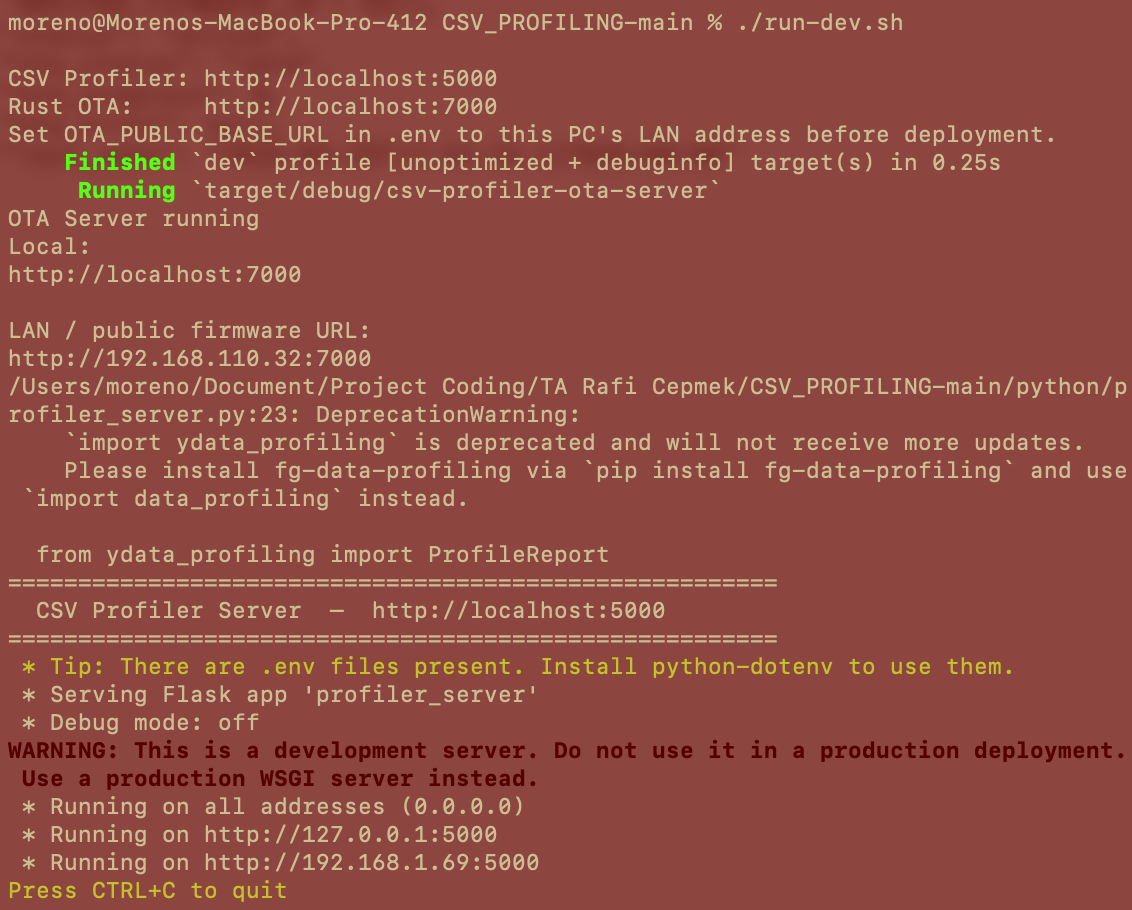
\includegraphics[width=0.88\textwidth]{ota_1.png}
  \caption{Output terminal saat \texttt{run-dev.sh} dijalankan --- Rust OTA Server
           dan Flask Profiler Server aktif bersamaan.}
  \label{fig:startup}
\end{figure}

%% ============================================================
\chapter{CSV Data Profiler}
%% ============================================================

\section{Gambaran Fitur}

CSV Data Profiler adalah antarmuka web yang memungkinkan pengguna mengunggah
dataset sensor dalam format CSV dan mendapatkan laporan analisis statistik secara
otomatis. Fitur yang tersedia meliputi:

\begin{itemize}[leftmargin=2cm, itemsep=2pt]
  \item Statistik deskriptif per variabel (mean, min, max, standar deviasi);
  \item Analisis korelasi antar variabel sensor;
  \item Deteksi nilai hilang (\textit{missing values});
  \item Inferensi tipe data otomatis;
  \item Grafik distribusi dan interaksi antar variabel.
\end{itemize}

\section{Tampilan Dashboard}

\begin{figure}[H]
  \centering
  \begin{subfigure}[b]{0.48\textwidth}
    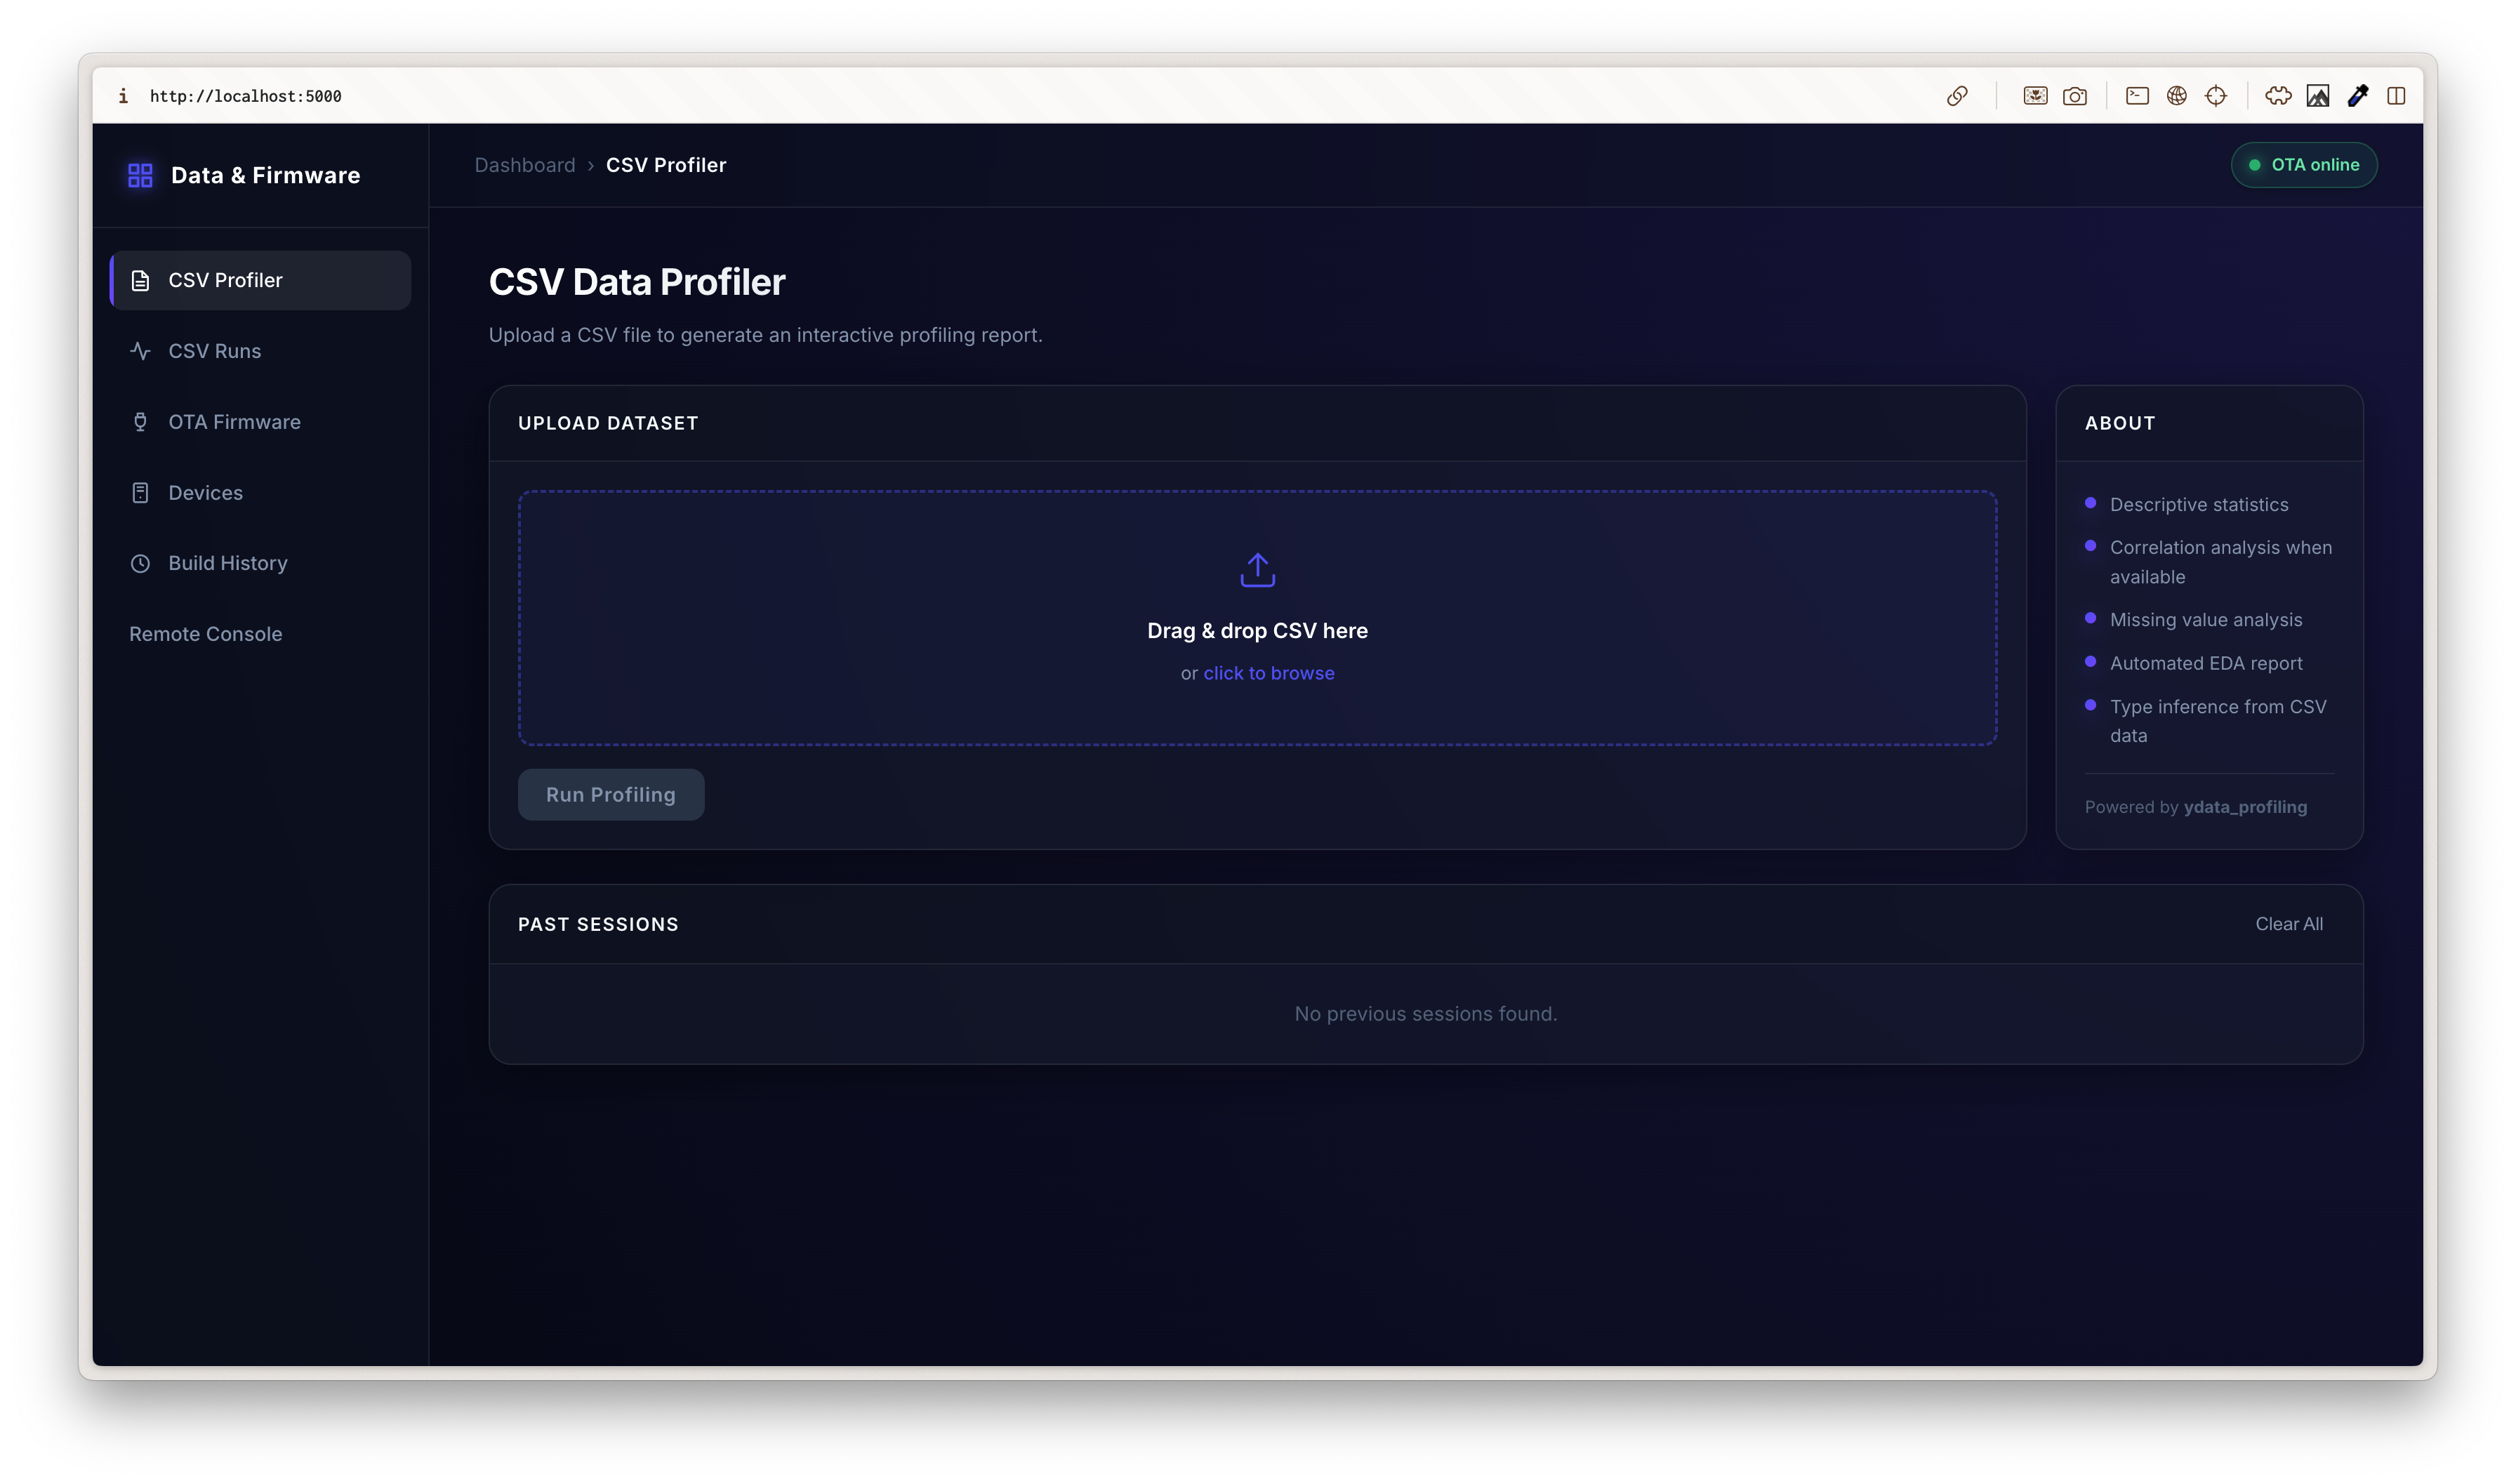
\includegraphics[width=\textwidth]{ota_3.png}
    \caption{Halaman CSV Profiler (upload dataset).}
    \label{fig:csvprofiler_a}
  \end{subfigure}
  \hfill
  \begin{subfigure}[b]{0.48\textwidth}
    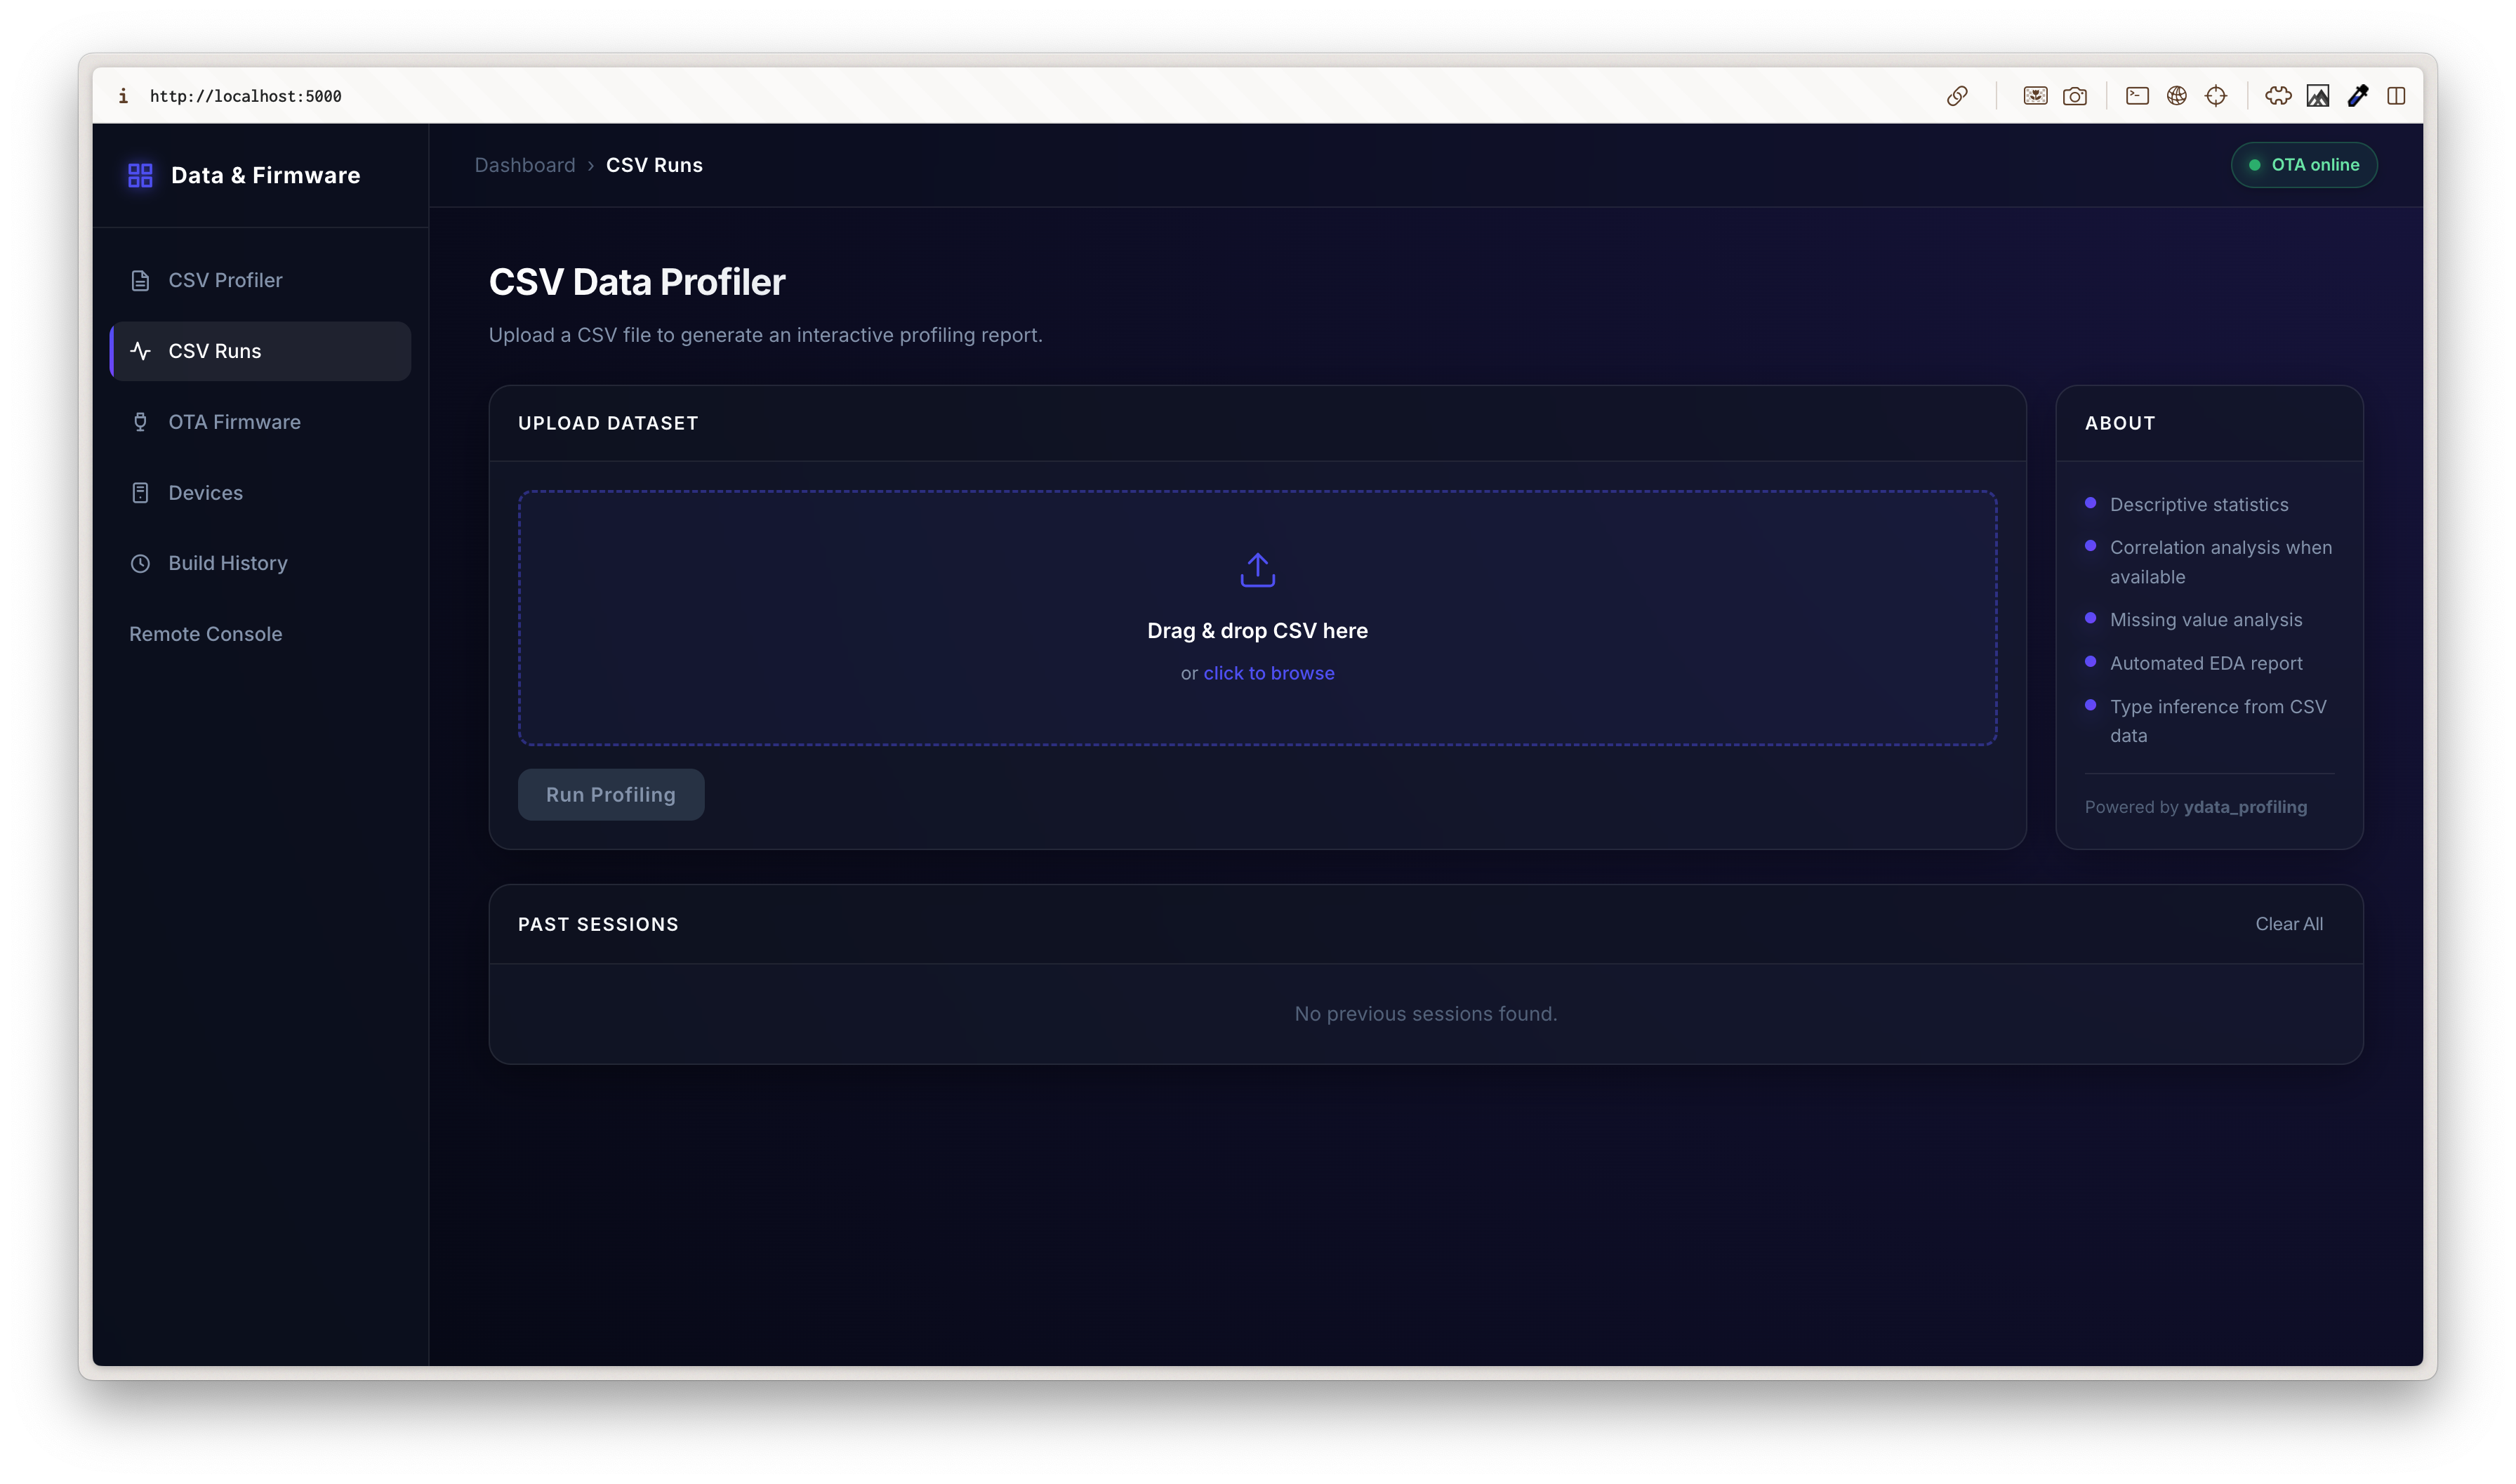
\includegraphics[width=\textwidth]{ota_4.png}
    \caption{Halaman CSV Runs (daftar sesi profiling).}
    \label{fig:csvprofiler_b}
  \end{subfigure}
  \caption{Antarmuka CSV Data Profiler pada \texttt{localhost:5000}.}
  \label{fig:csvprofiler}
\end{figure}

\begin{figure}[H]
  \centering
  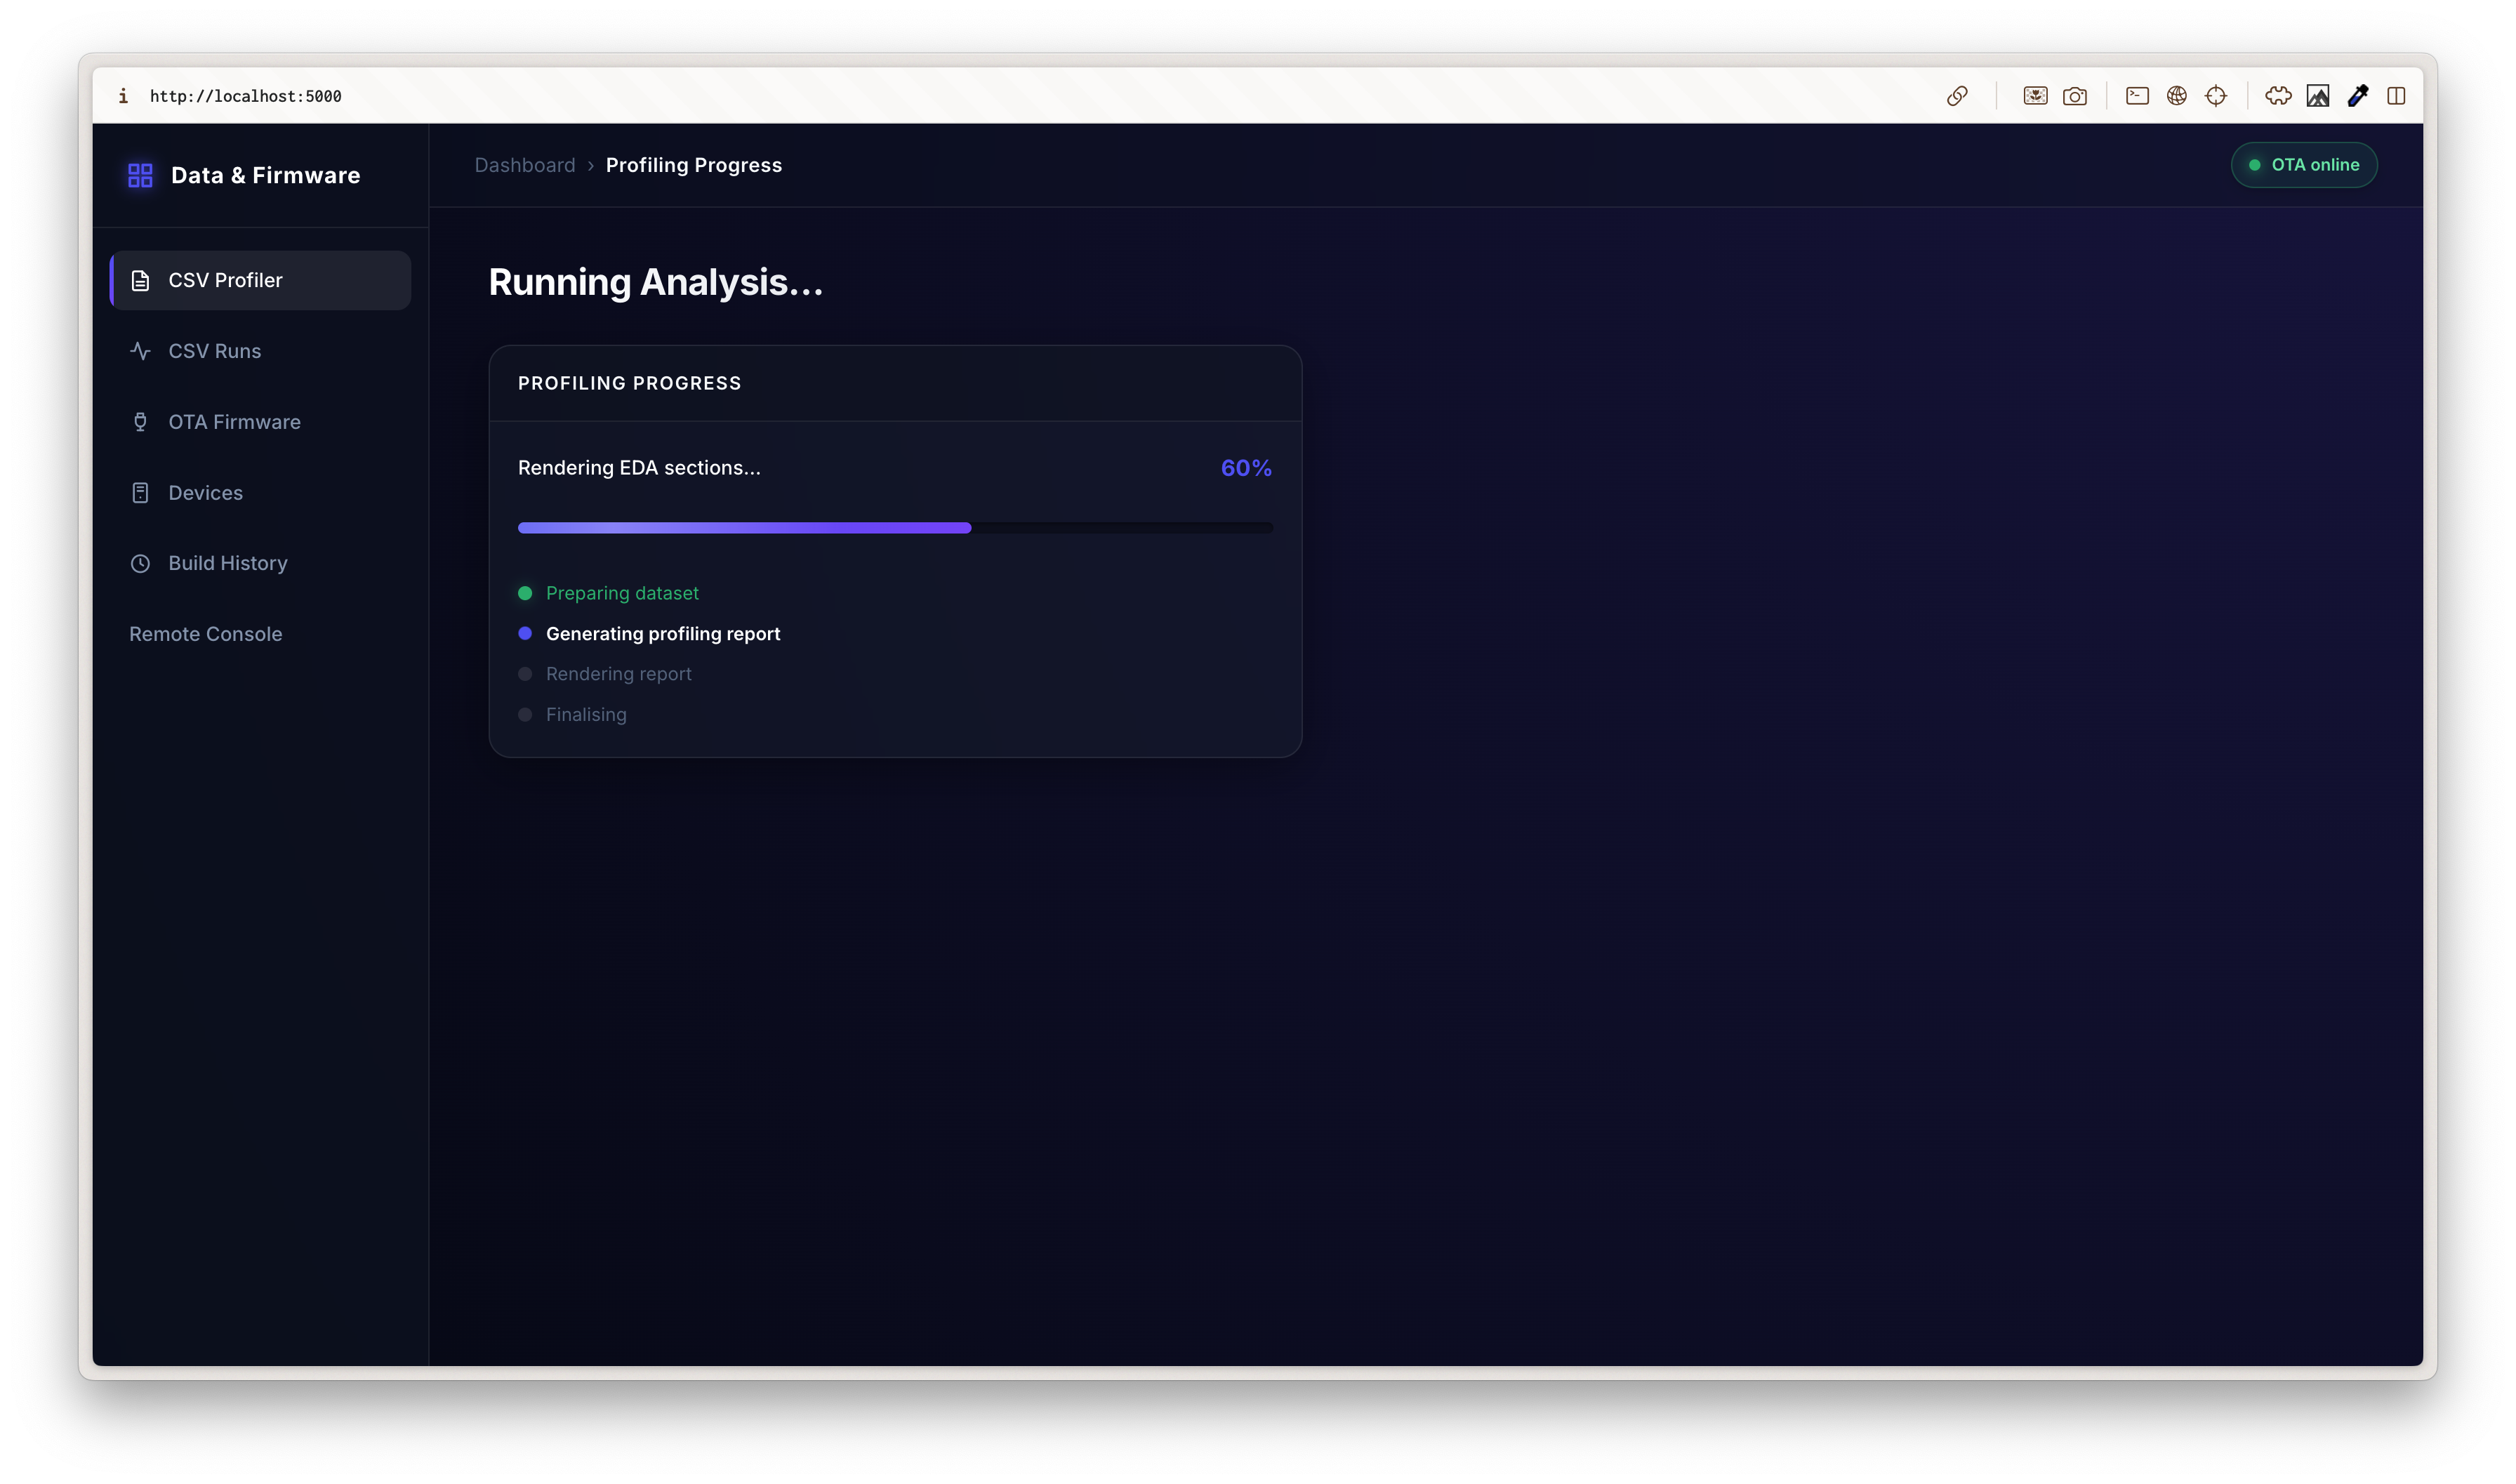
\includegraphics[width=0.6\textwidth]{ota_9.png}
  \caption{Proses profiling sedang berjalan --- tampilan progress 60\% pada fase
           \textit{Generating profiling report}.}
  \label{fig:profiling_progress}
\end{figure}

\section{Hasil Profiling Dataset Sensor}

Dataset yang digunakan dalam pengujian merupakan data simulasi sensor gas E-Nose
selama satu siklus pengujian (300 detik, 300 observasi). Dataset mengandung
\textbf{9 variabel} (1 kolom waktu + 8 sensor gas) dengan \textbf{300 baris} data.

\subsection{Ikhtisar Dataset}

\begin{figure}[H]
  \centering
  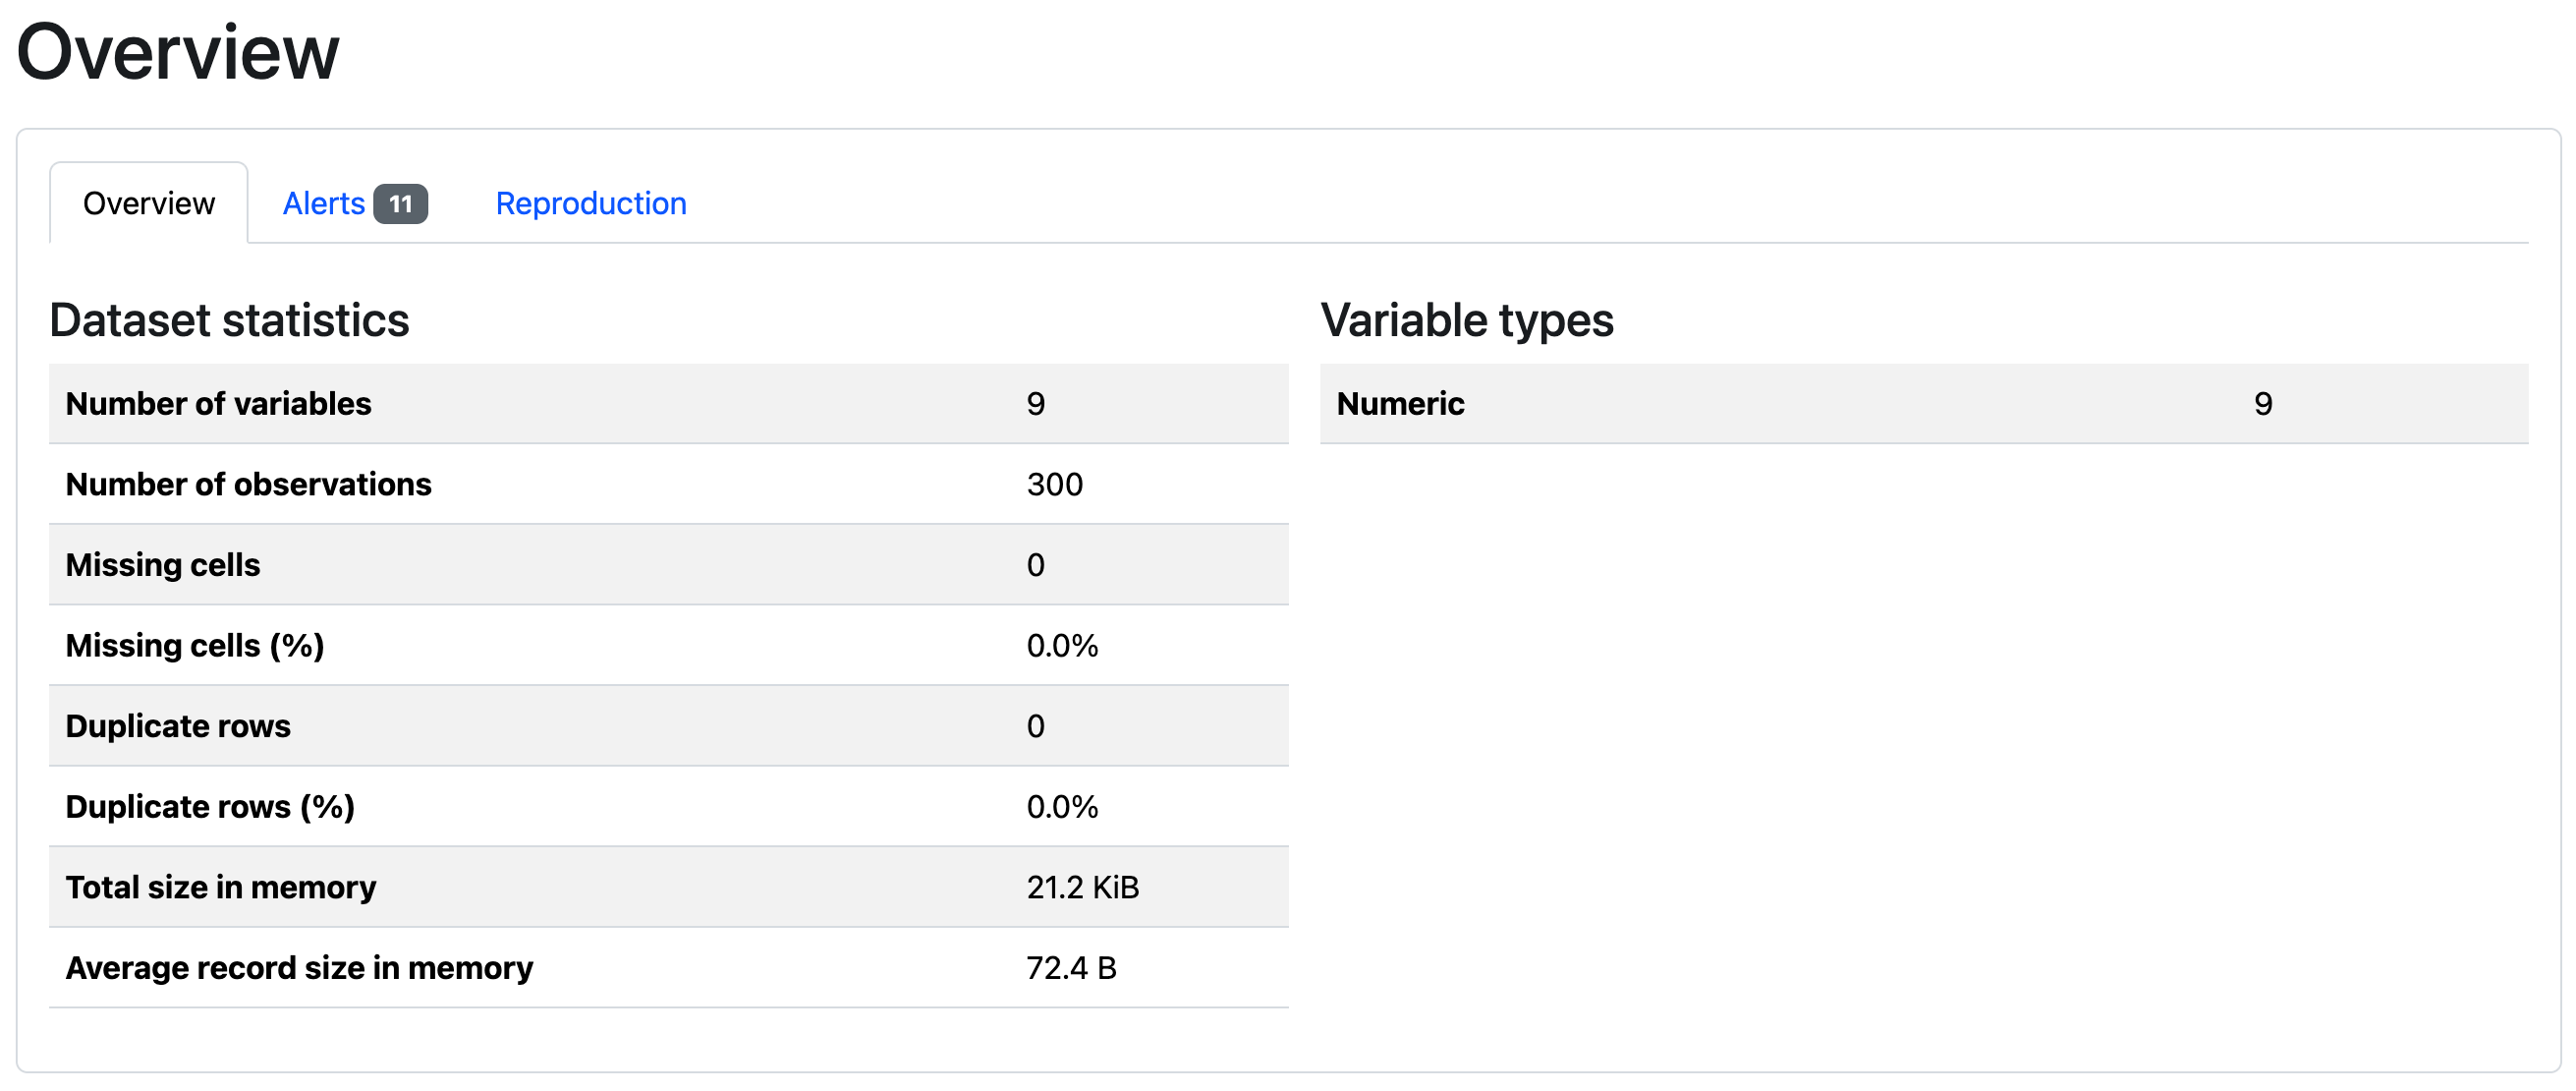
\includegraphics[width=0.88\textwidth]{profiling_1.png}
  \caption{Ikhtisar statistik dataset --- 9 variabel, 300 observasi,
           0 nilai hilang, 0 baris duplikat.}
  \label{fig:profiling_overview}
\end{figure}

Hasil profiling menunjukkan bahwa dataset dalam kondisi \textbf{bersih} sempurna:
tidak terdapat nilai hilang (\textit{missing values}) maupun baris duplikat,
sehingga data siap digunakan untuk analisis lebih lanjut.

\begin{table}[H]
  \centering
  \caption{Statistik ringkasan dataset sensor E-Nose.}
  \label{tab:dataset_stats}
  \begin{tabular}{lc}
    \toprule
    \textbf{Properti} & \textbf{Nilai} \\
    \midrule
    Jumlah variabel    & 9 \\
    Jumlah observasi   & 300 \\
    Nilai hilang       & 0 (0.0\%) \\
    Baris duplikat     & 0 (0.0\%) \\
    Ukuran total memori & 21.2 KiB \\
    Ukuran rata-rata per baris & 72.4 B \\
    Tipe variabel      & Numerik semua \\
    \bottomrule
  \end{tabular}
\end{table}

\subsection{Profil Per Variabel Sensor}

Berikut adalah contoh profil statistik untuk dua sensor representatif.

\begin{figure}[H]
  \centering
  \begin{subfigure}[b]{0.48\textwidth}
    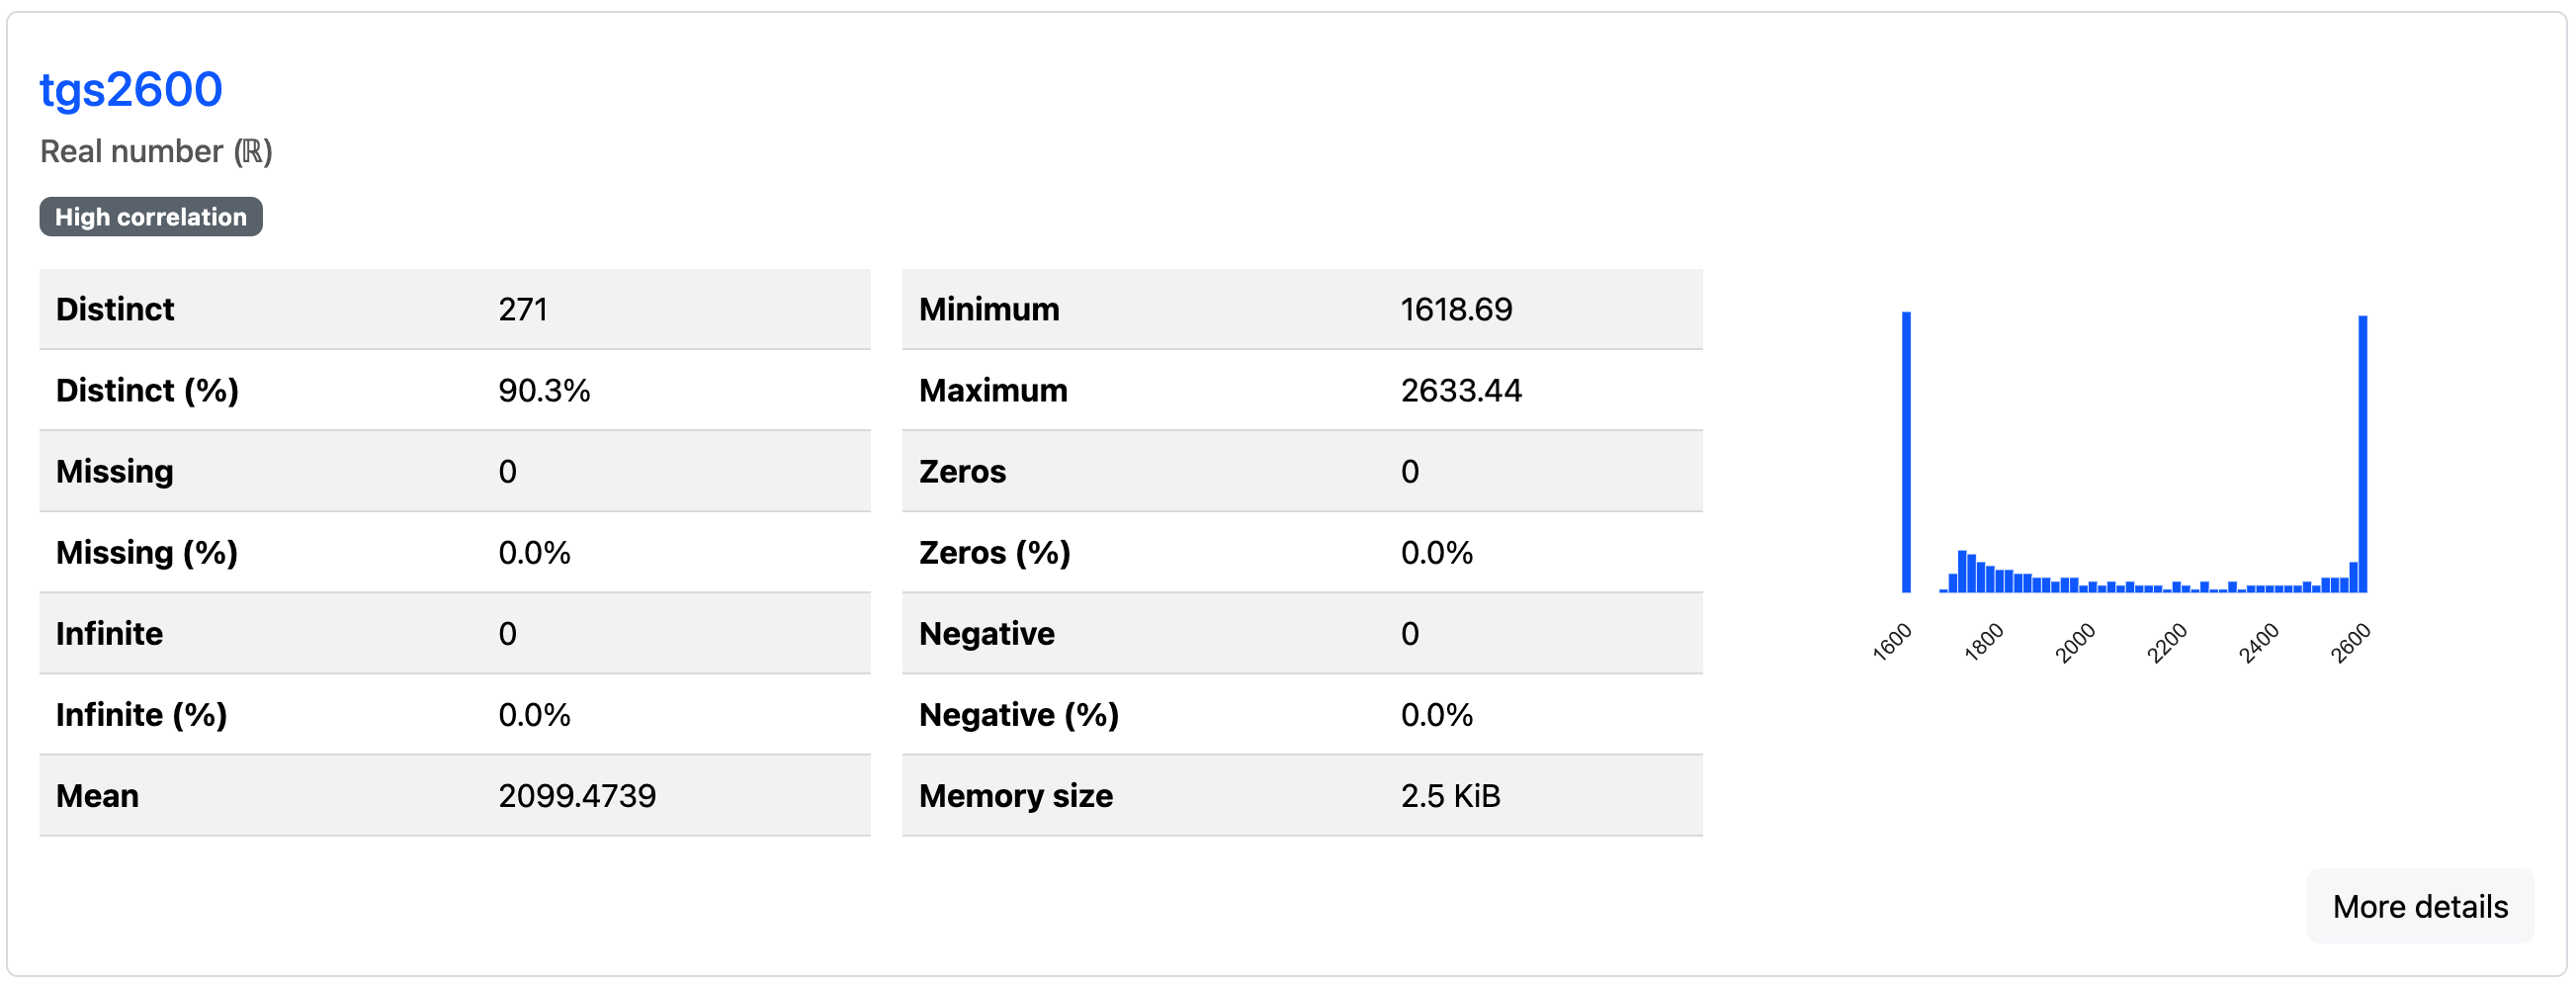
\includegraphics[width=\textwidth]{profiling_2.png}
    \caption{Profil variabel \texttt{tgs2600}.}
    \label{fig:var_tgs2600}
  \end{subfigure}
  \hfill
  \begin{subfigure}[b]{0.48\textwidth}
    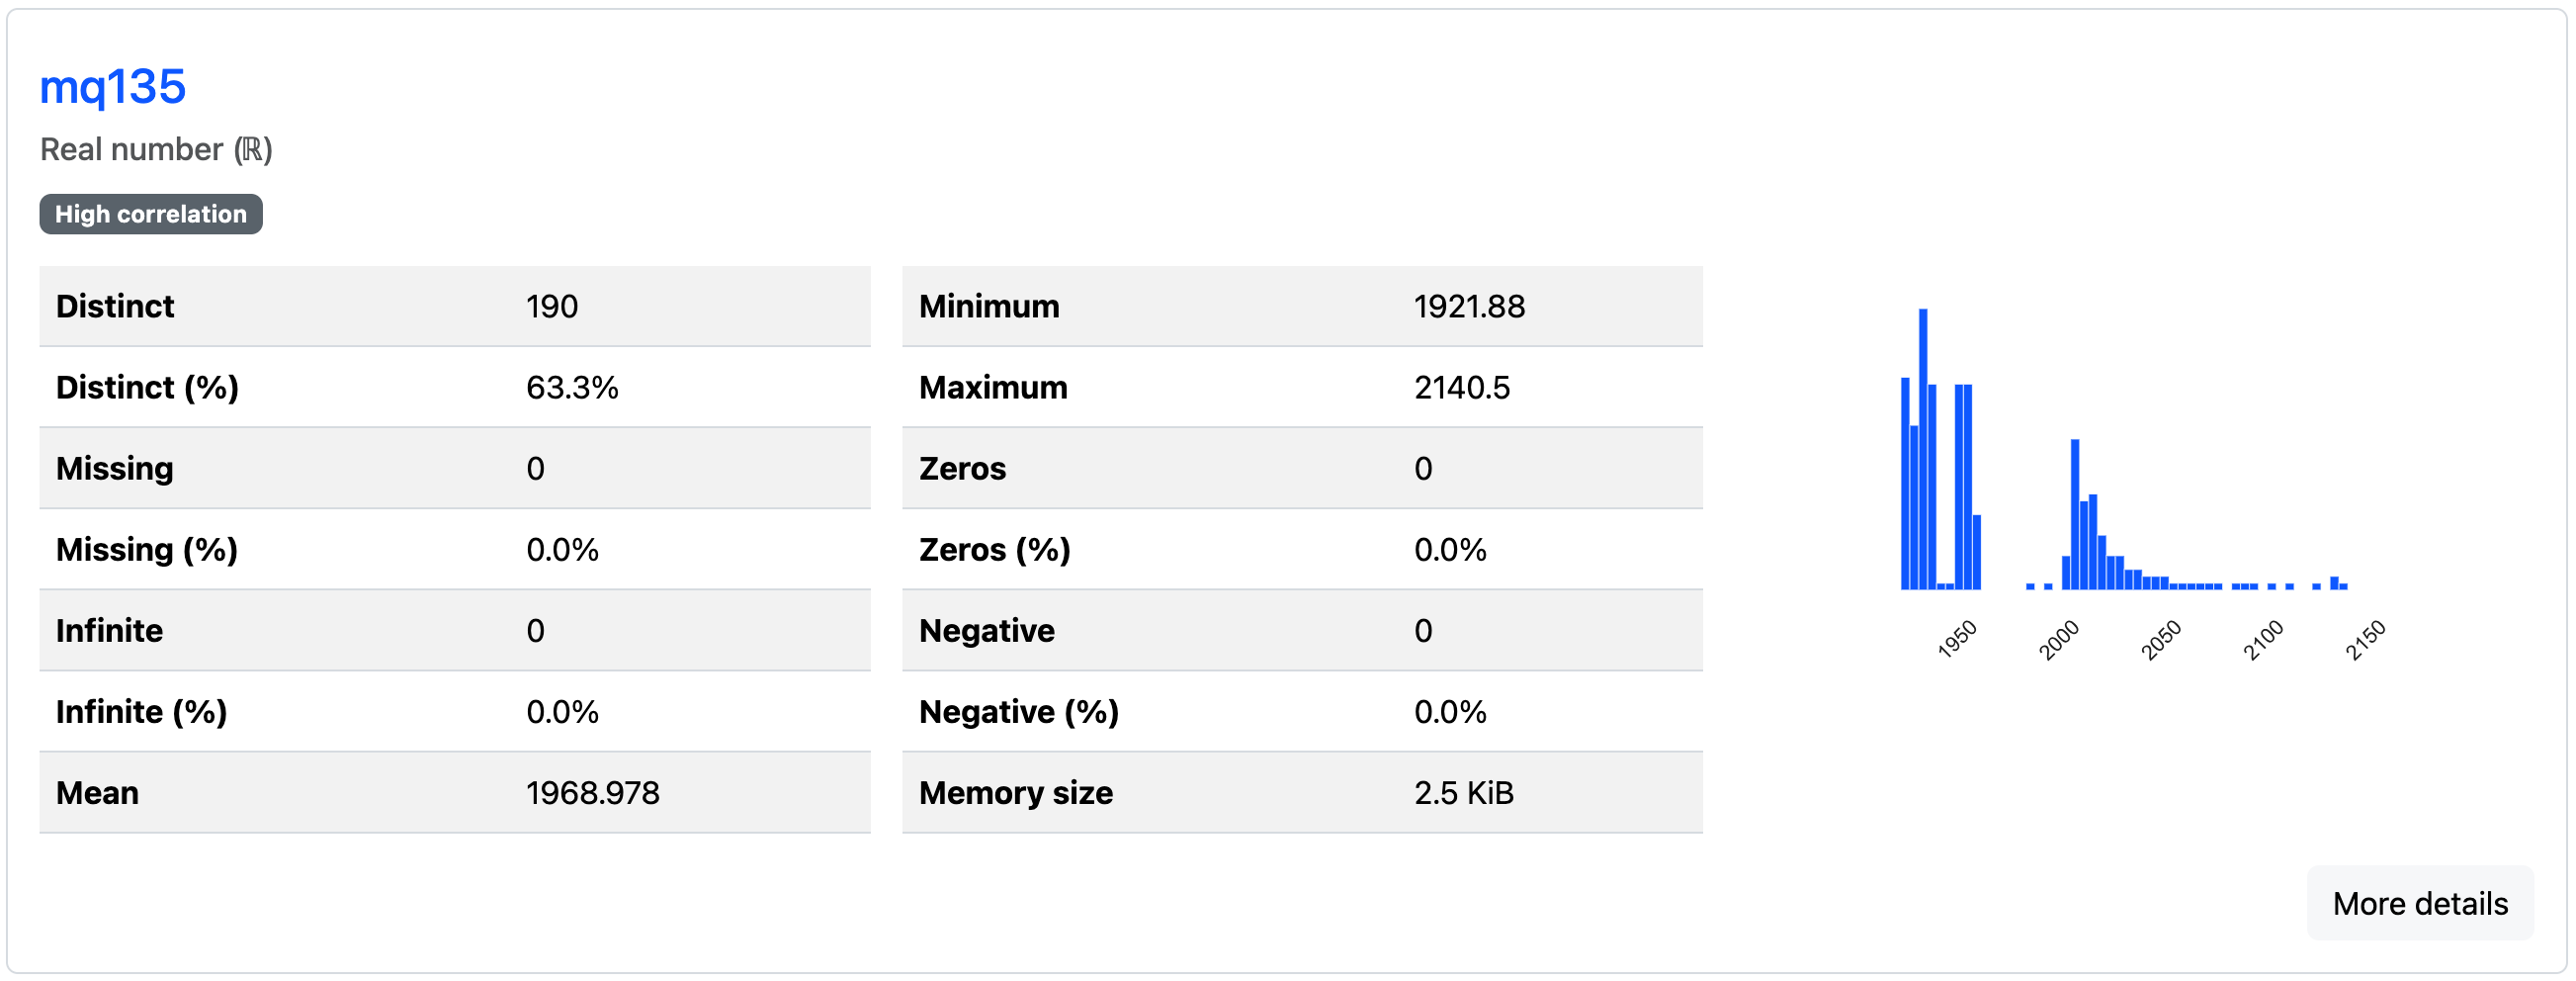
\includegraphics[width=\textwidth]{profiling_3.png}
    \caption{Profil variabel \texttt{mq135}.}
    \label{fig:var_mq135}
  \end{subfigure}
  \caption{Profil statistik sensor TGS2600 dan MQ-135.}
  \label{fig:var_profil}
\end{figure}

Sensor TGS2600 memiliki rentang nilai \textbf{1618.69 -- 2633.44 mV} dengan
rata-rata 2099.47 mV, sementara sensor MQ-135 berkisar pada
\textbf{1921.88 -- 2140.5 mV} dengan rata-rata 1968.98 mV.

\subsection{Matriks Korelasi}

\begin{figure}[H]
  \centering
  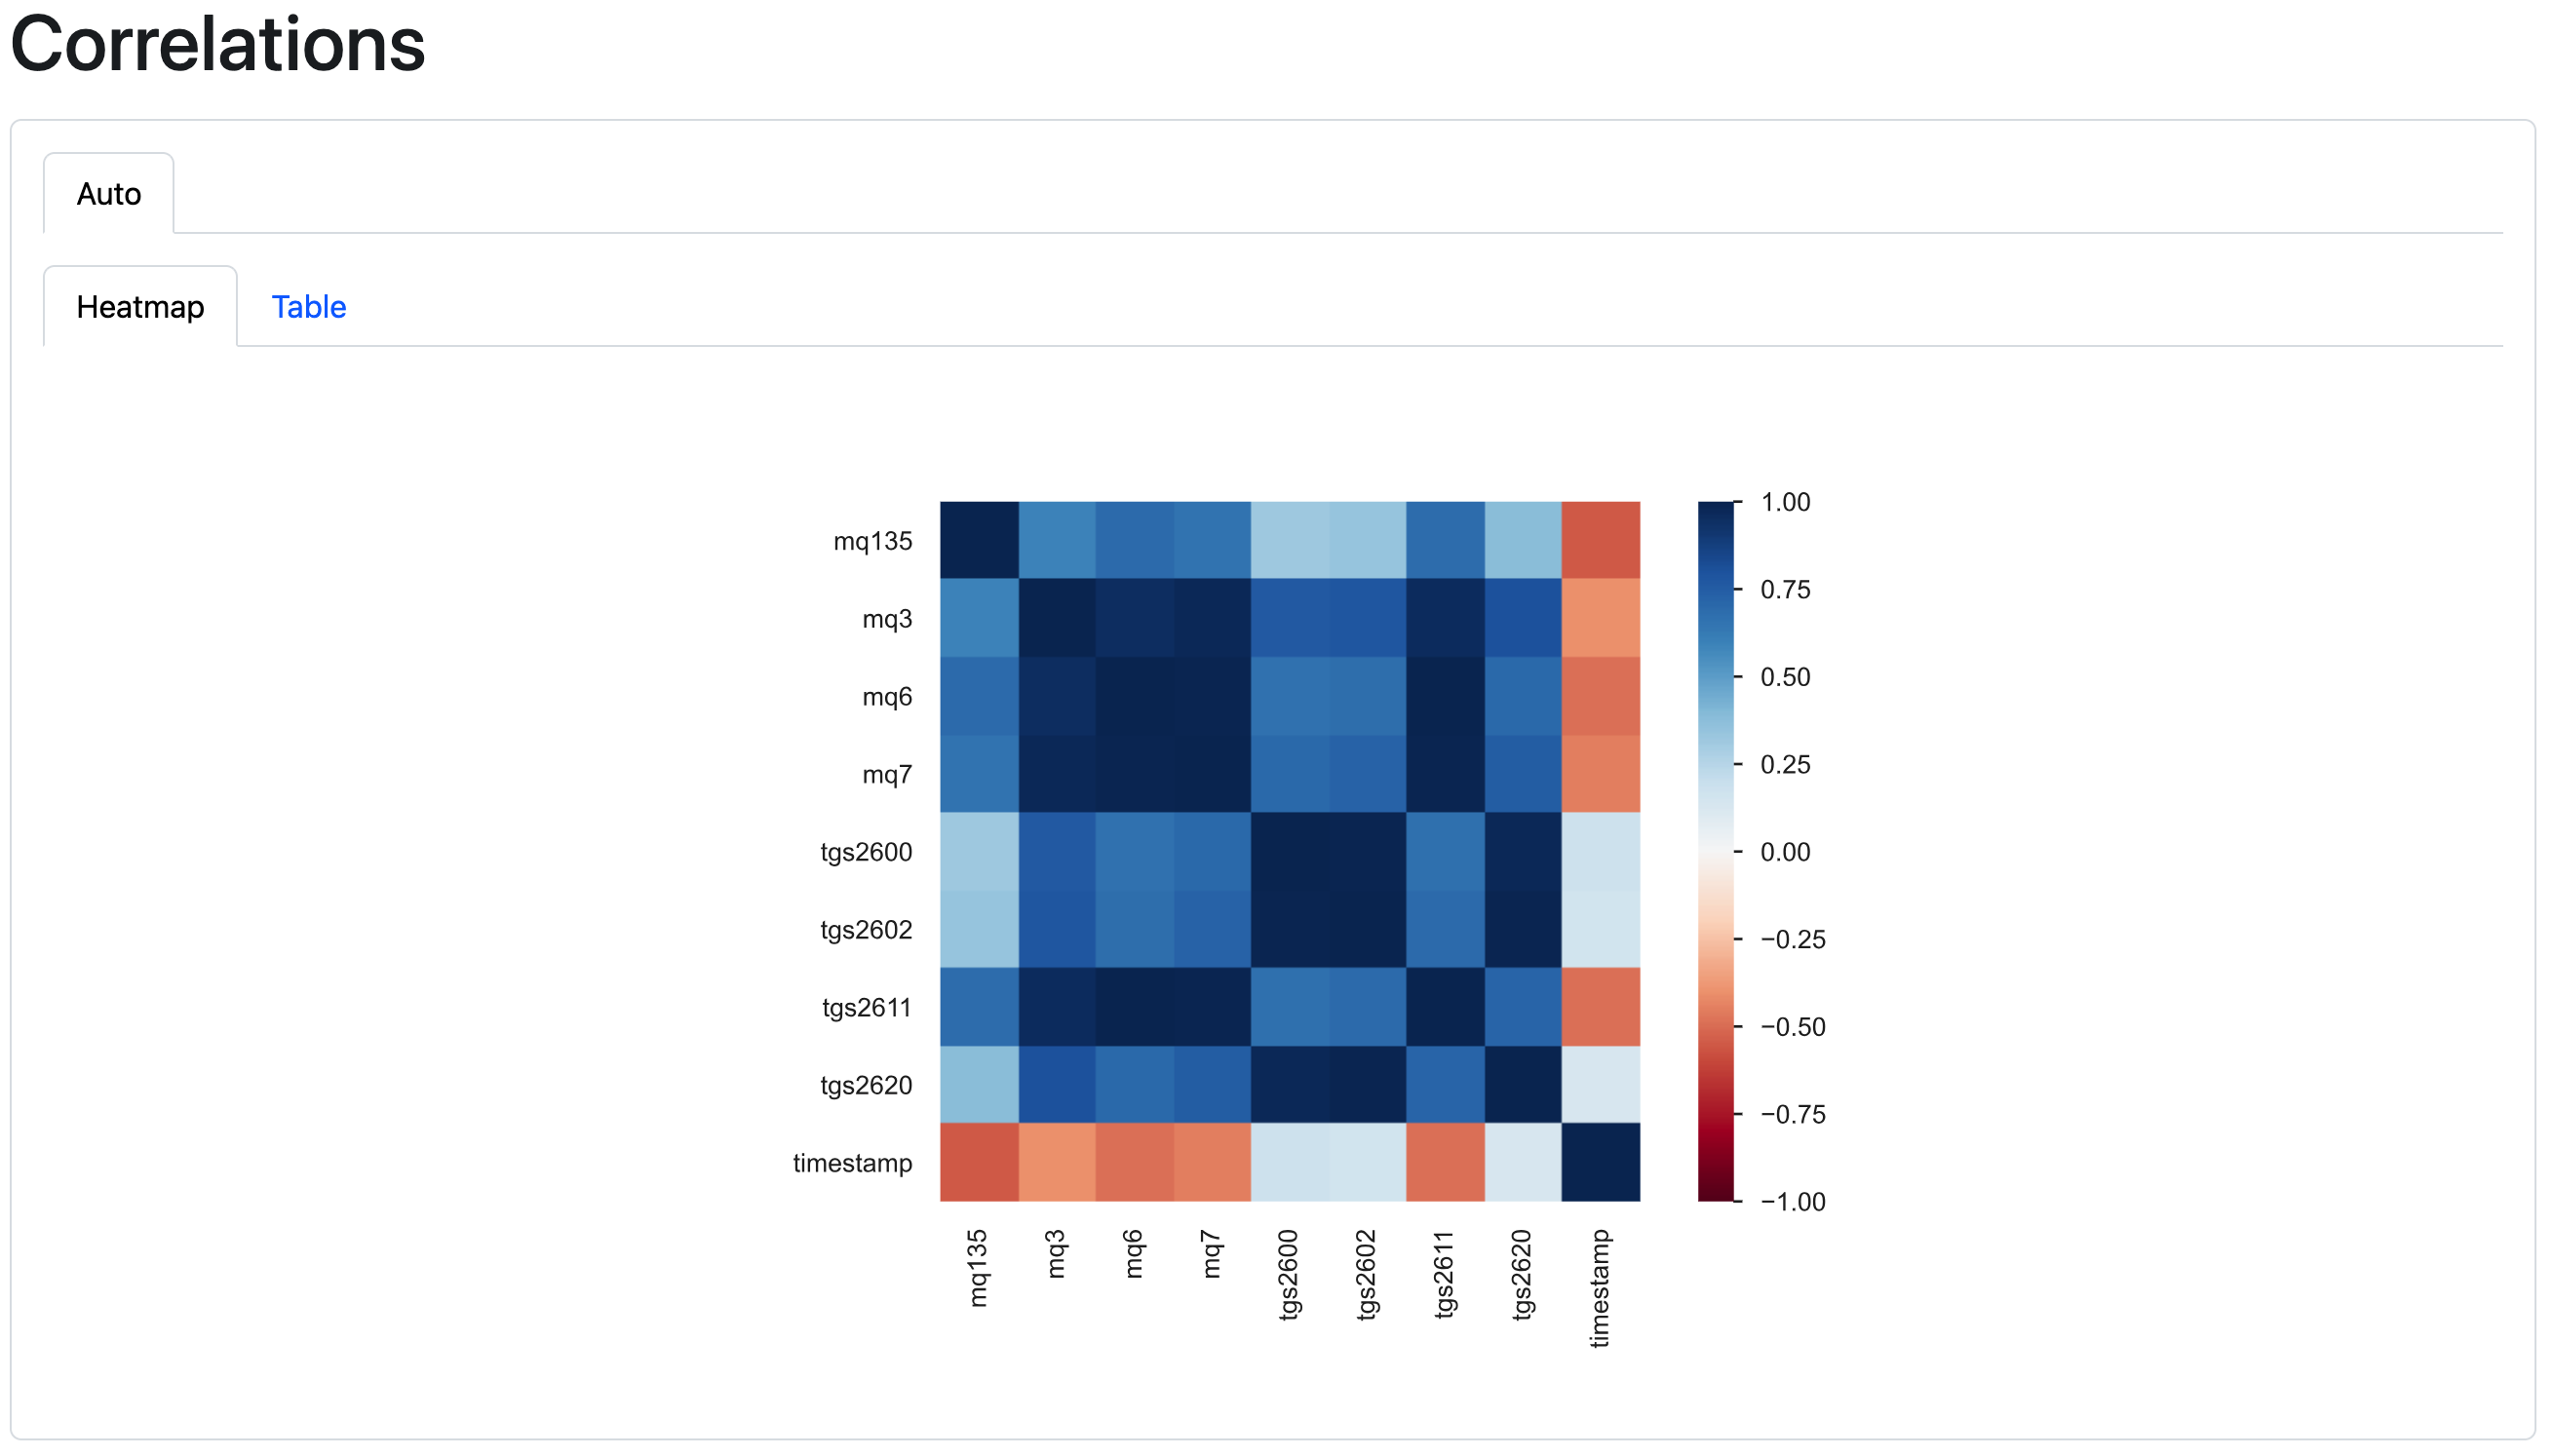
\includegraphics[width=0.72\textwidth]{profiling_11.png}
  \caption{Heatmap korelasi otomatis antar variabel sensor.}
  \label{fig:correlasi}
\end{figure}

Heatmap korelasi menunjukkan bahwa sebagian besar sensor gas (MQ dan TGS)
\textbf{berkorelasi positif satu sama lain}, yang konsisten dengan sifat fisik
sensor gas yang merespons konsentrasi gas secara bersamaan dalam satu chamber.

\subsection{Analisis Interaksi Antar Variabel}

\begin{figure}[H]
  \centering
  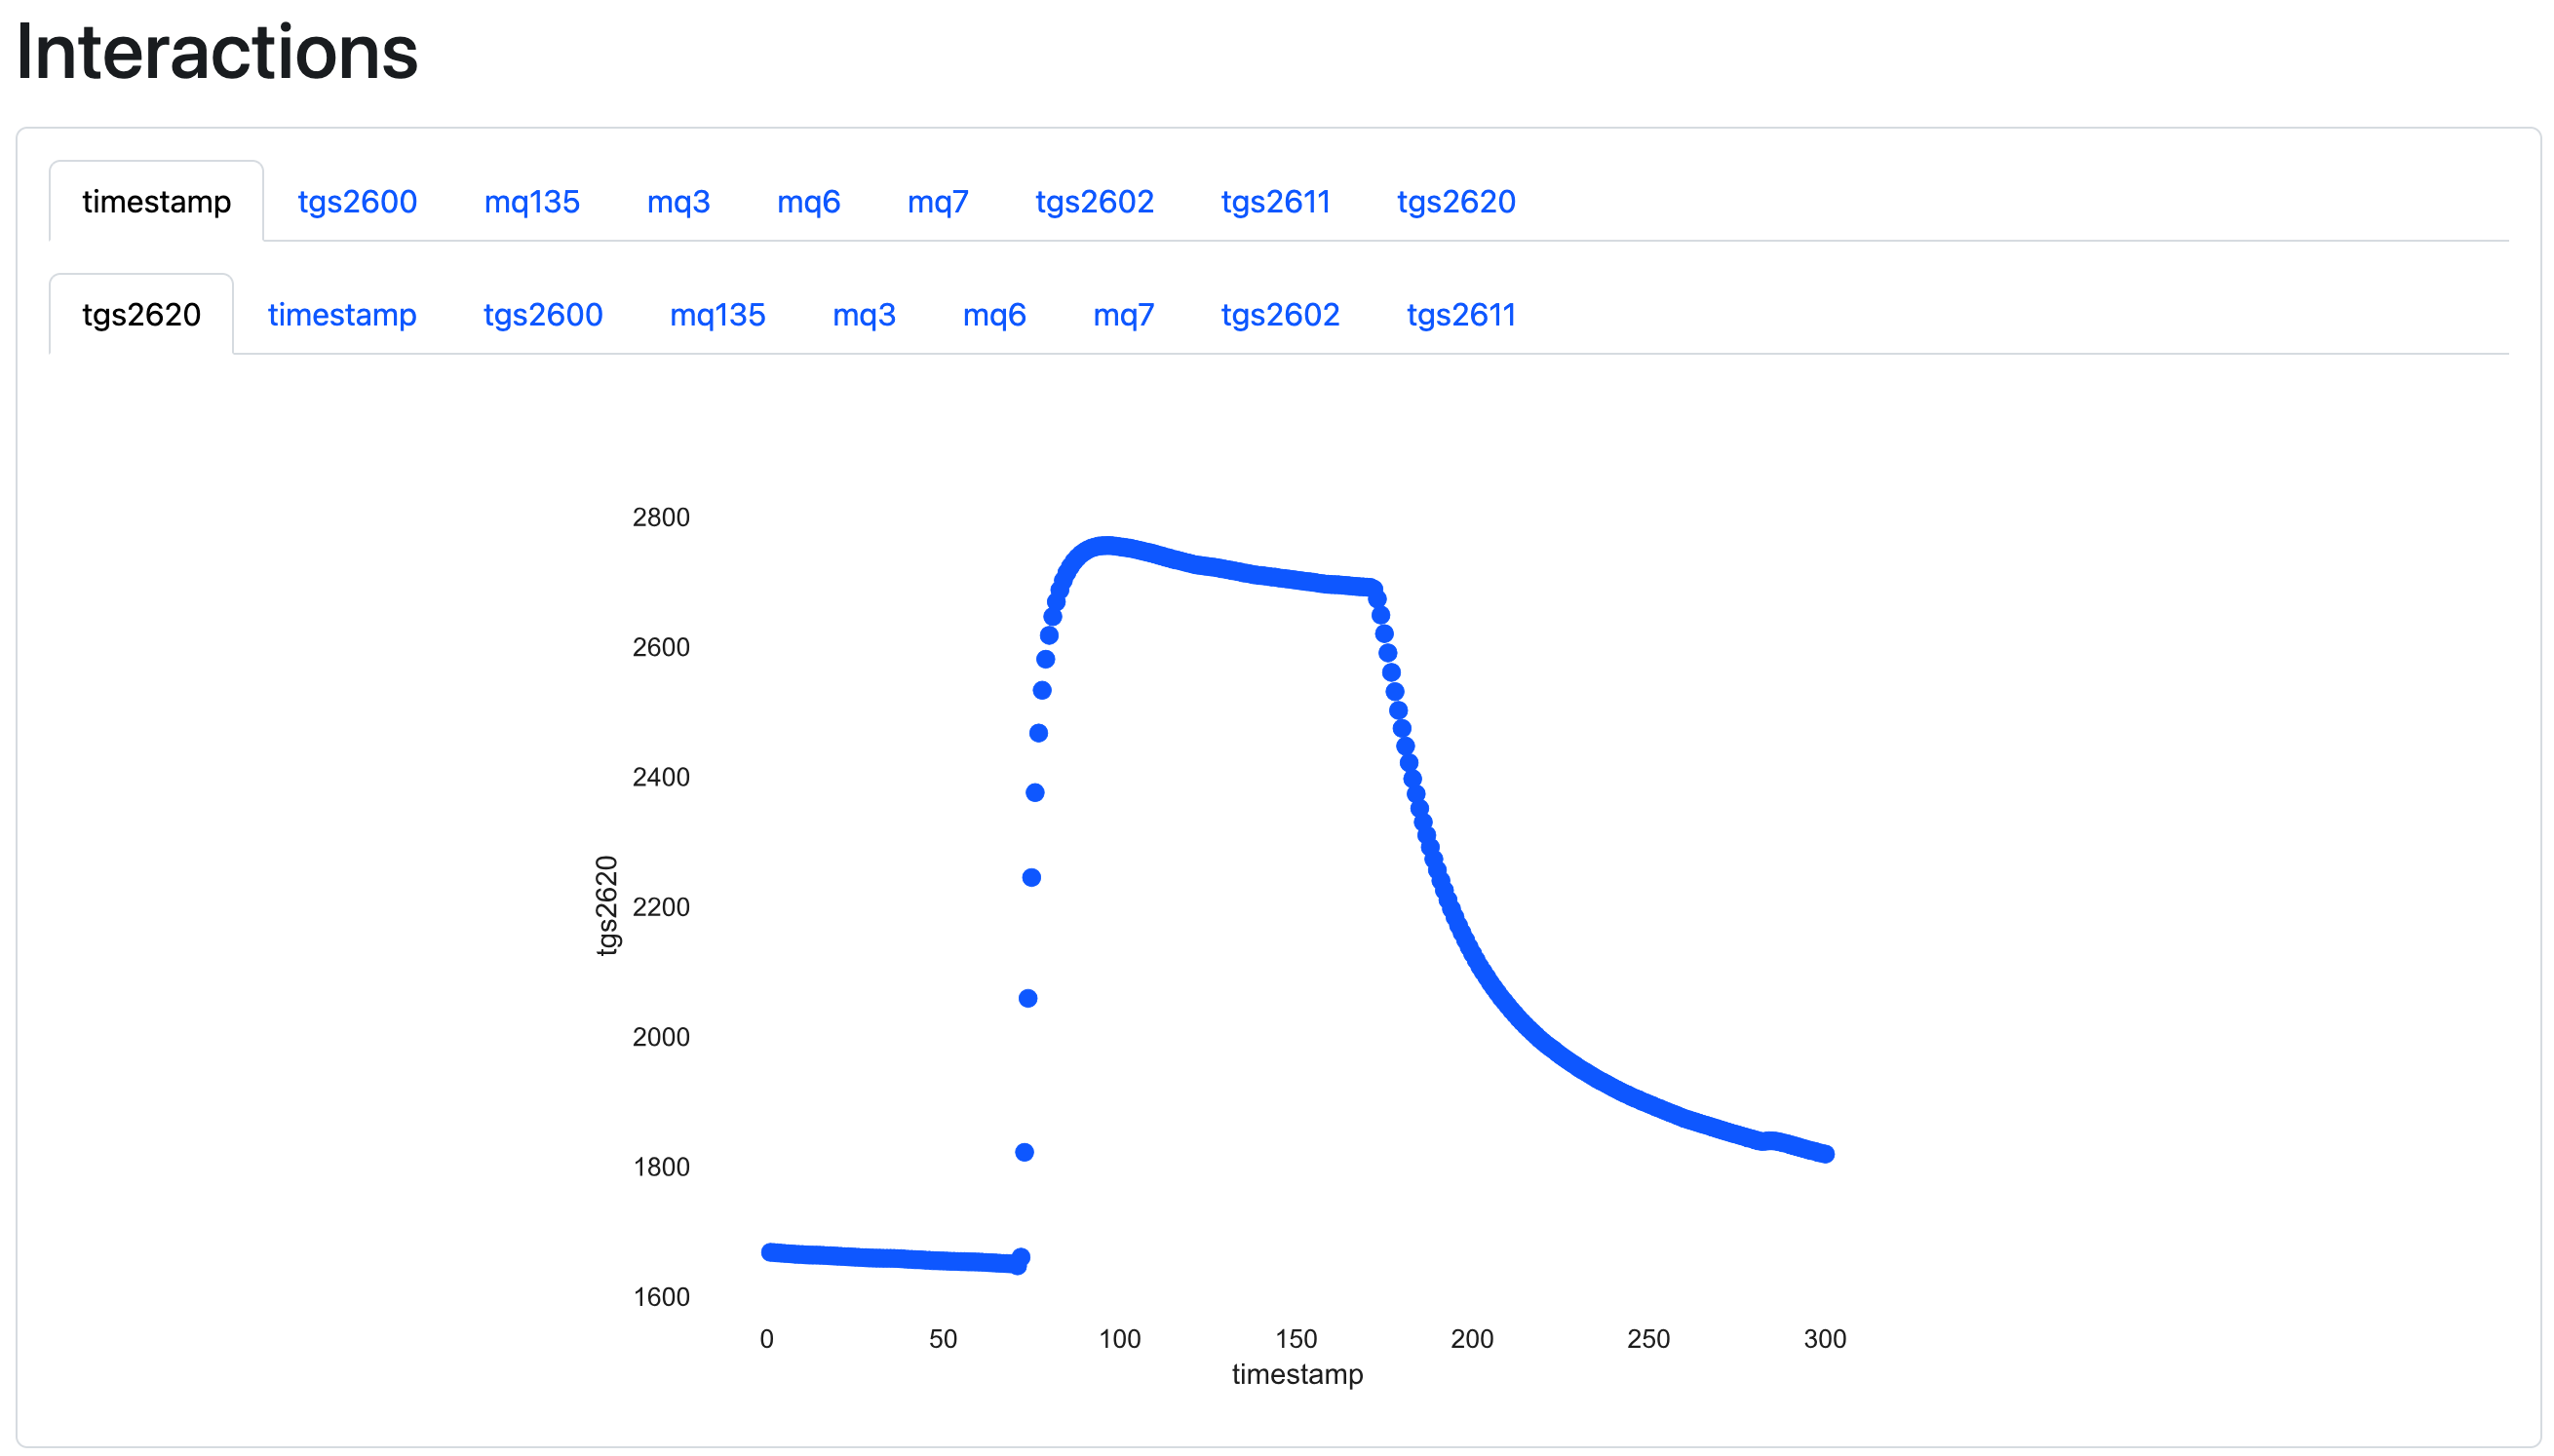
\includegraphics[width=0.8\textwidth]{profiling_10.png}
  \caption{Grafik interaksi \texttt{tgs2620} terhadap \texttt{timestamp}.}
  \label{fig:interaksi}
\end{figure}

Grafik interaksi menampilkan \textbf{pola kurva eksponensial} yang khas: nilai
sensor naik tajam saat fase inlet dan turun bertahap saat fase outlet.

\subsection{Analisis Nilai Hilang}

\begin{figure}[H]
  \centering
  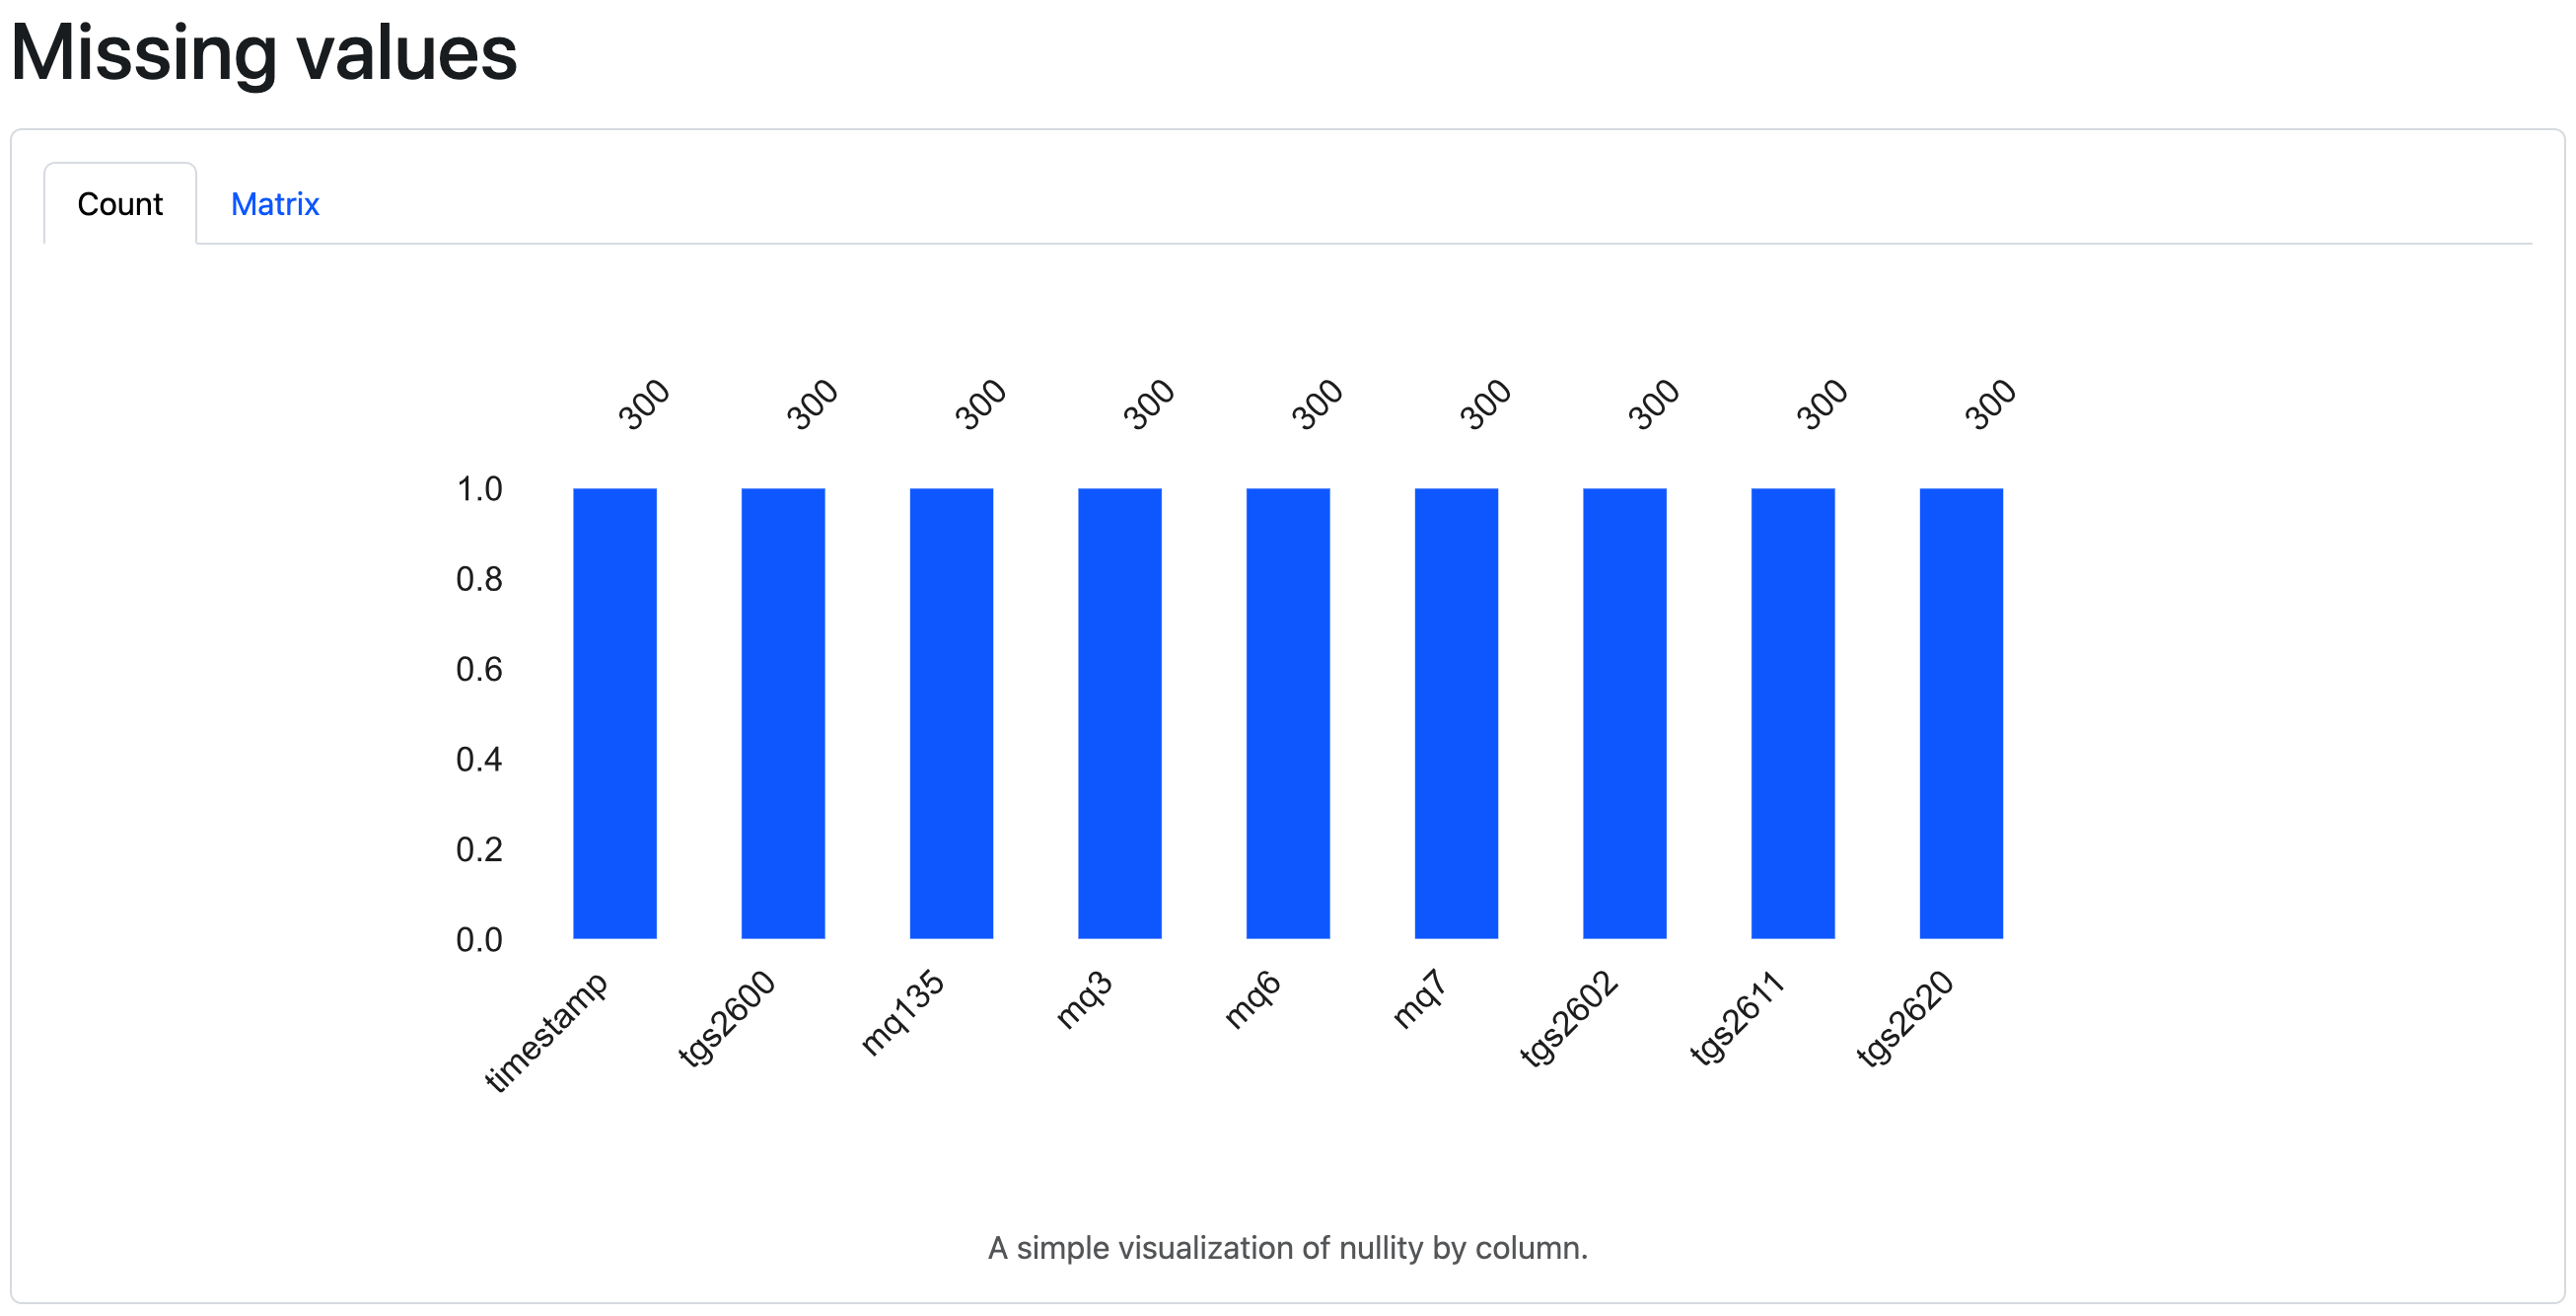
\includegraphics[width=0.82\textwidth]{profiling_12.png}
  \caption{Visualisasi \textit{missing values} --- semua 9 variabel memiliki
           300 nilai lengkap (0\% hilang).}
  \label{fig:missing}
\end{figure}

\subsection{Sampel Data}

\begin{figure}[H]
  \centering
  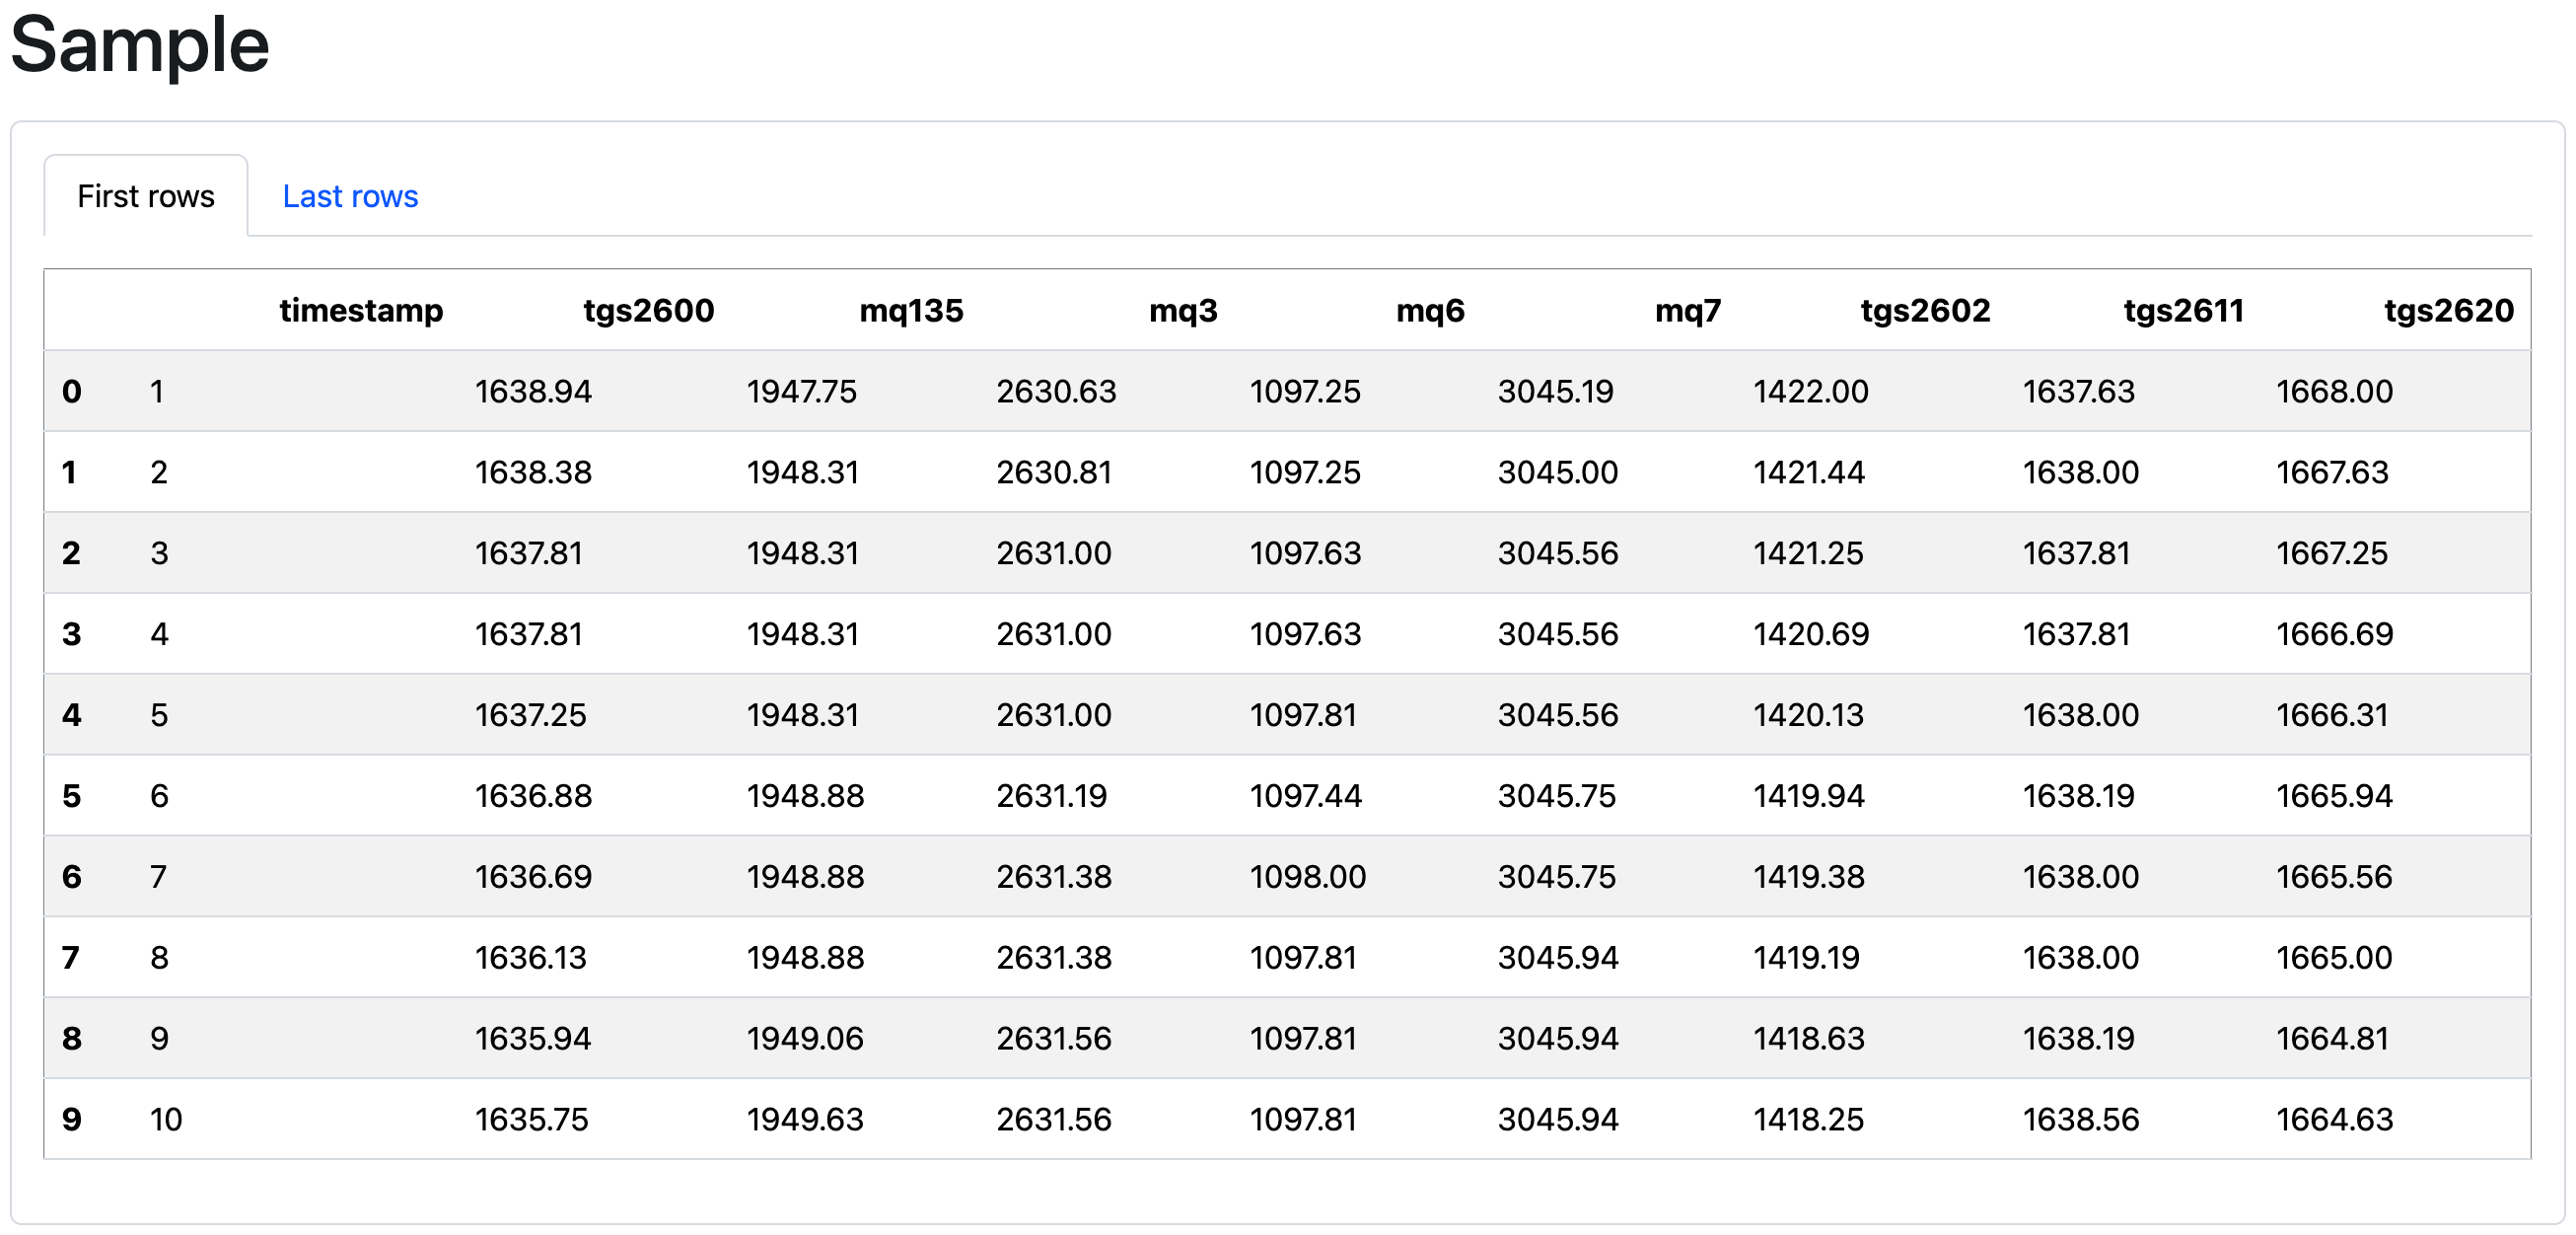
\includegraphics[width=0.95\textwidth]{profiling_13.png}
  \caption{Sepuluh baris pertama dataset sensor E-Nose.}
  \label{fig:sample_data}
\end{figure}

%% ============================================================
\chapter{OTA Firmware Server}
%% ============================================================

\section{Gambaran Fitur}

OTA (\textit{Over-The-Air}) Firmware Server dibangun menggunakan bahasa
\textbf{Rust} dengan \textit{framework} Axum. Server ini menyediakan antarmuka
terpadu untuk manajemen \textit{firmware} ESP32.

\begin{infobox}{Akses OTA Server}
  OTA Server berjalan pada \textbf{\texttt{http://localhost:7000}} (API backend)
  dan dapat diakses melalui dashboard web di \textbf{\texttt{http://localhost:5000}}.
\end{infobox}

\section{Halaman OTA Firmware (Build \& Upload)}

\begin{figure}[H]
  \centering
  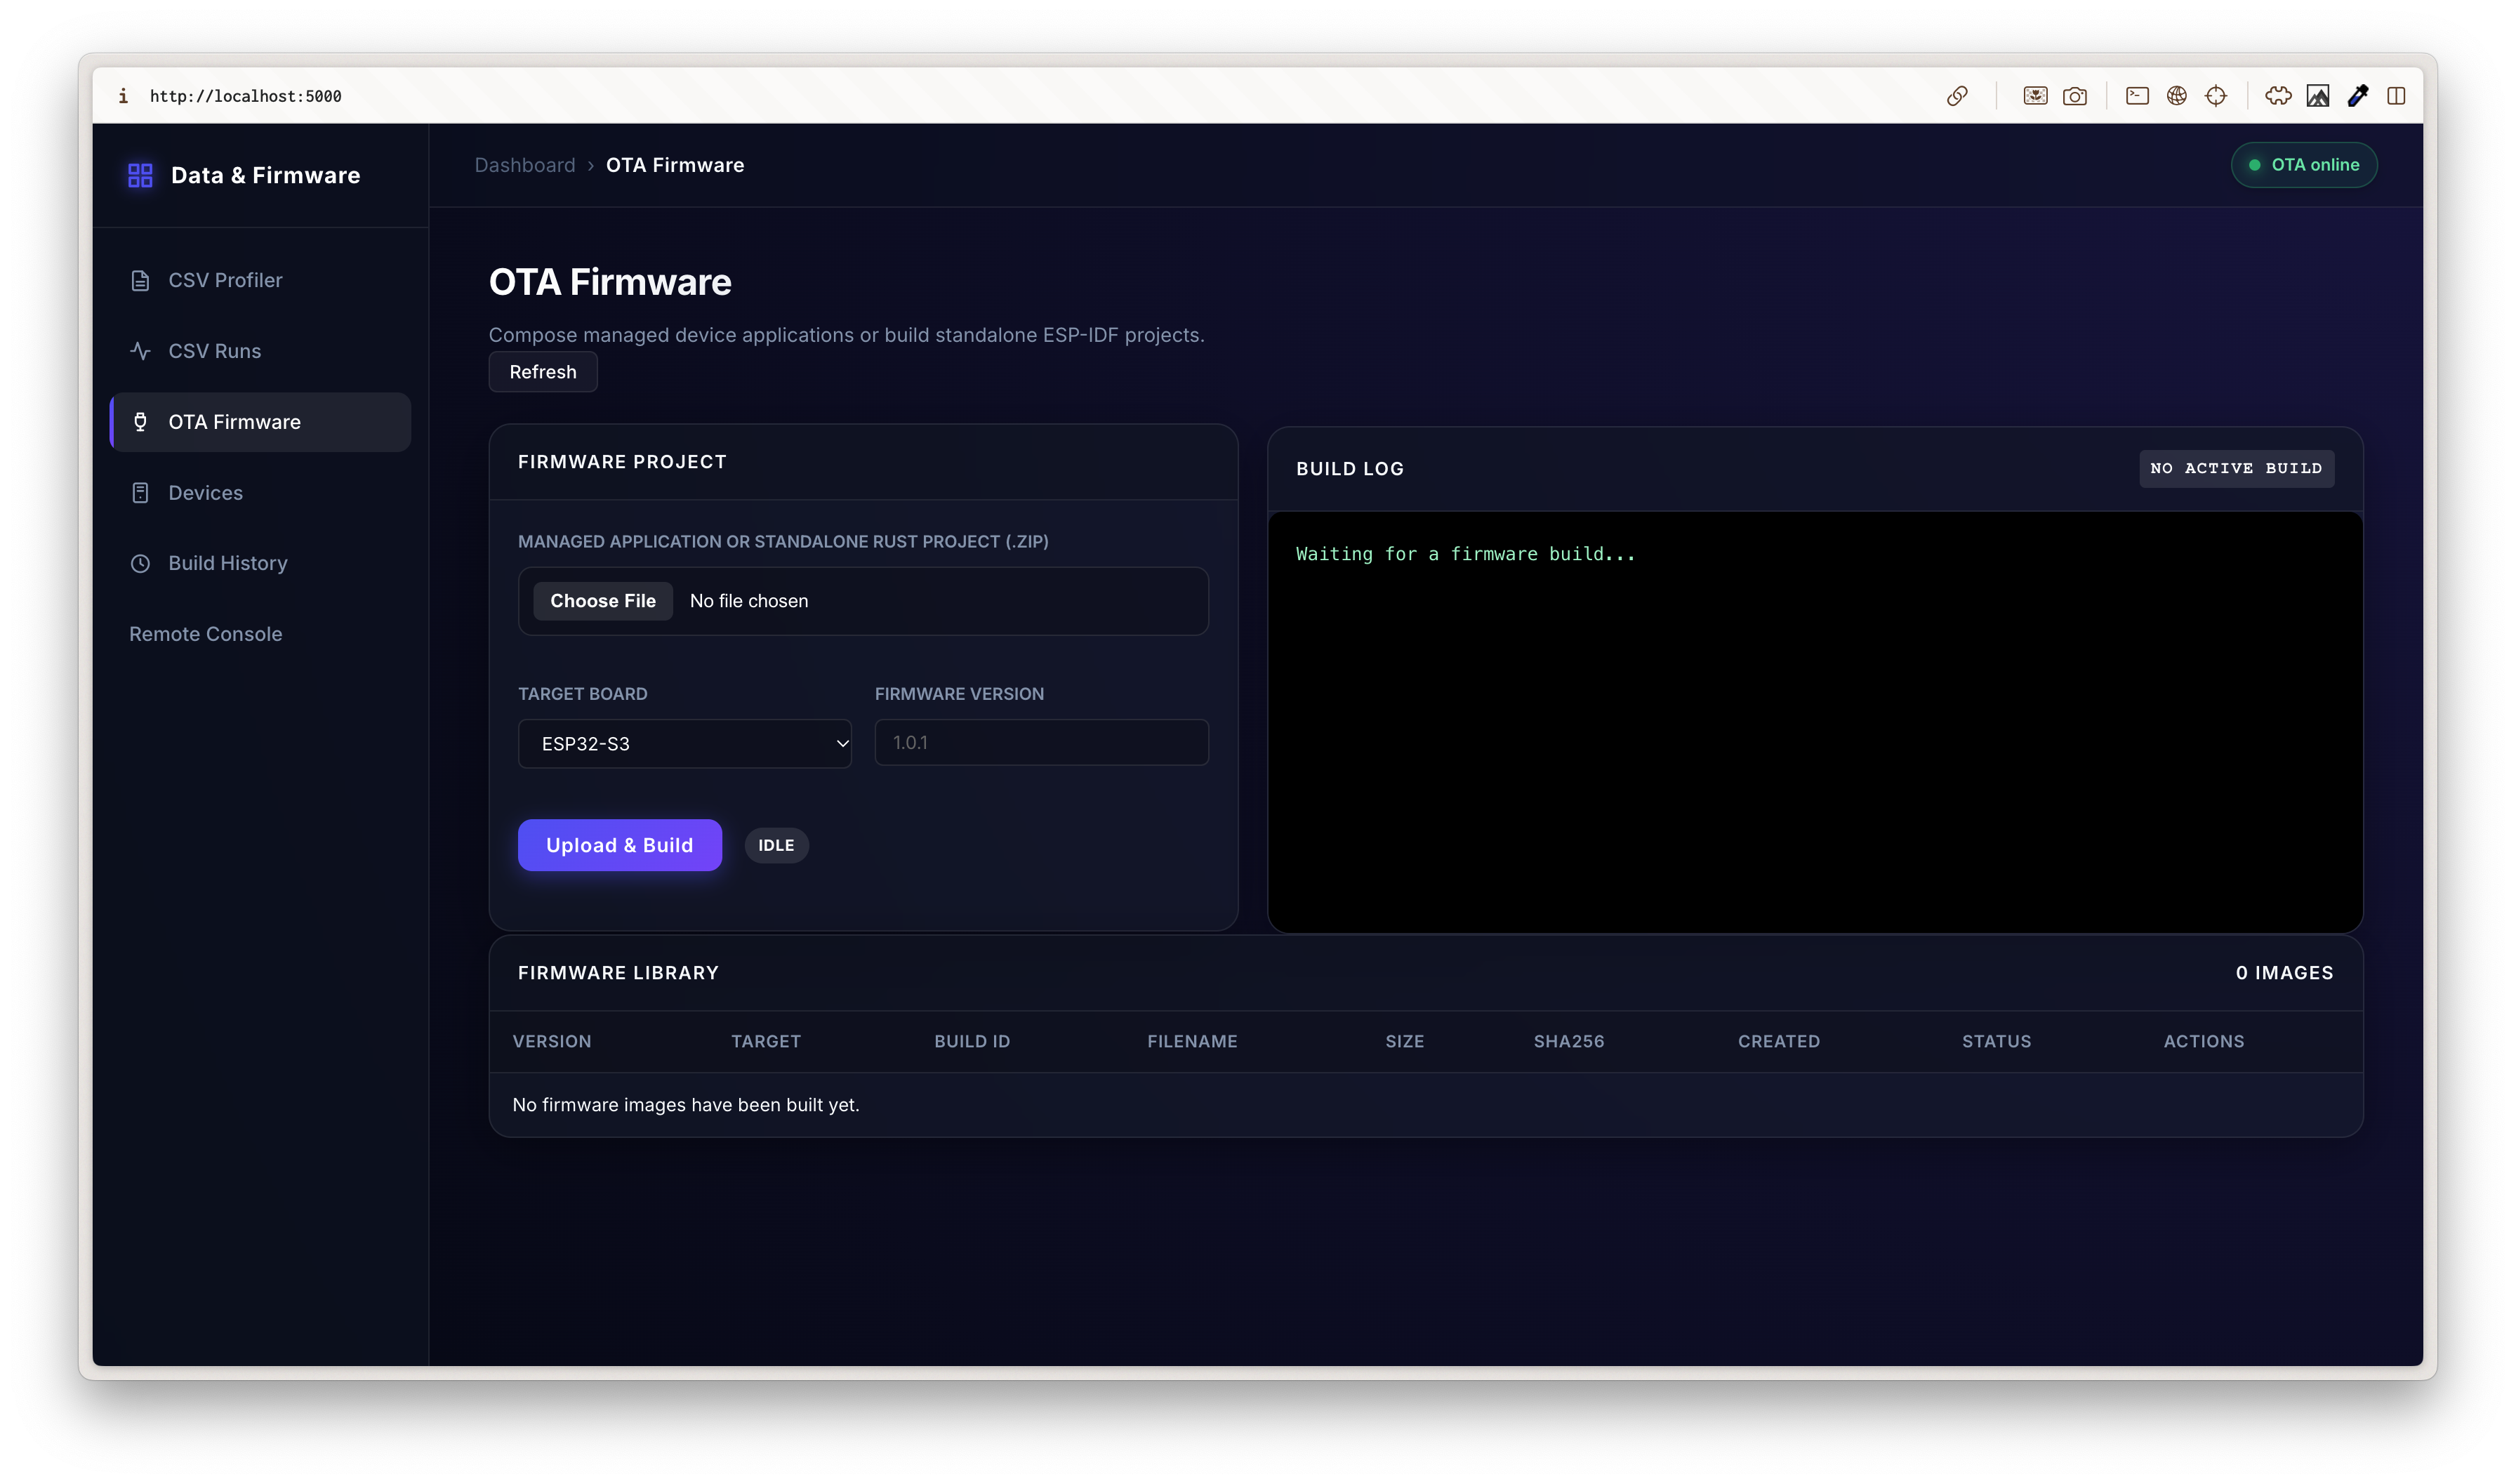
\includegraphics[width=0.88\textwidth]{ota_5.png}
  \caption{Halaman OTA Firmware --- upload proyek dan build log real-time.}
  \label{fig:ota_firmware}
\end{figure}

Halaman ini menyediakan:
\begin{itemize}[leftmargin=2cm, itemsep=2pt]
  \item \textbf{Upload file} proyek firmware (\texttt{.zip});
  \item Pemilihan \textbf{Target Board} (ESP32-S3, ESP32, dll.);
  \item Penentuan \textbf{Firmware Version};
  \item Tombol \textbf{Upload \& Build};
  \item \textbf{Build Log} \textit{real-time};
  \item \textbf{Firmware Library} --- tabel semua \textit{image} yang telah di-build.
\end{itemize}

\section{Halaman Manajemen Perangkat (Devices)}

\begin{figure}[H]
  \centering
  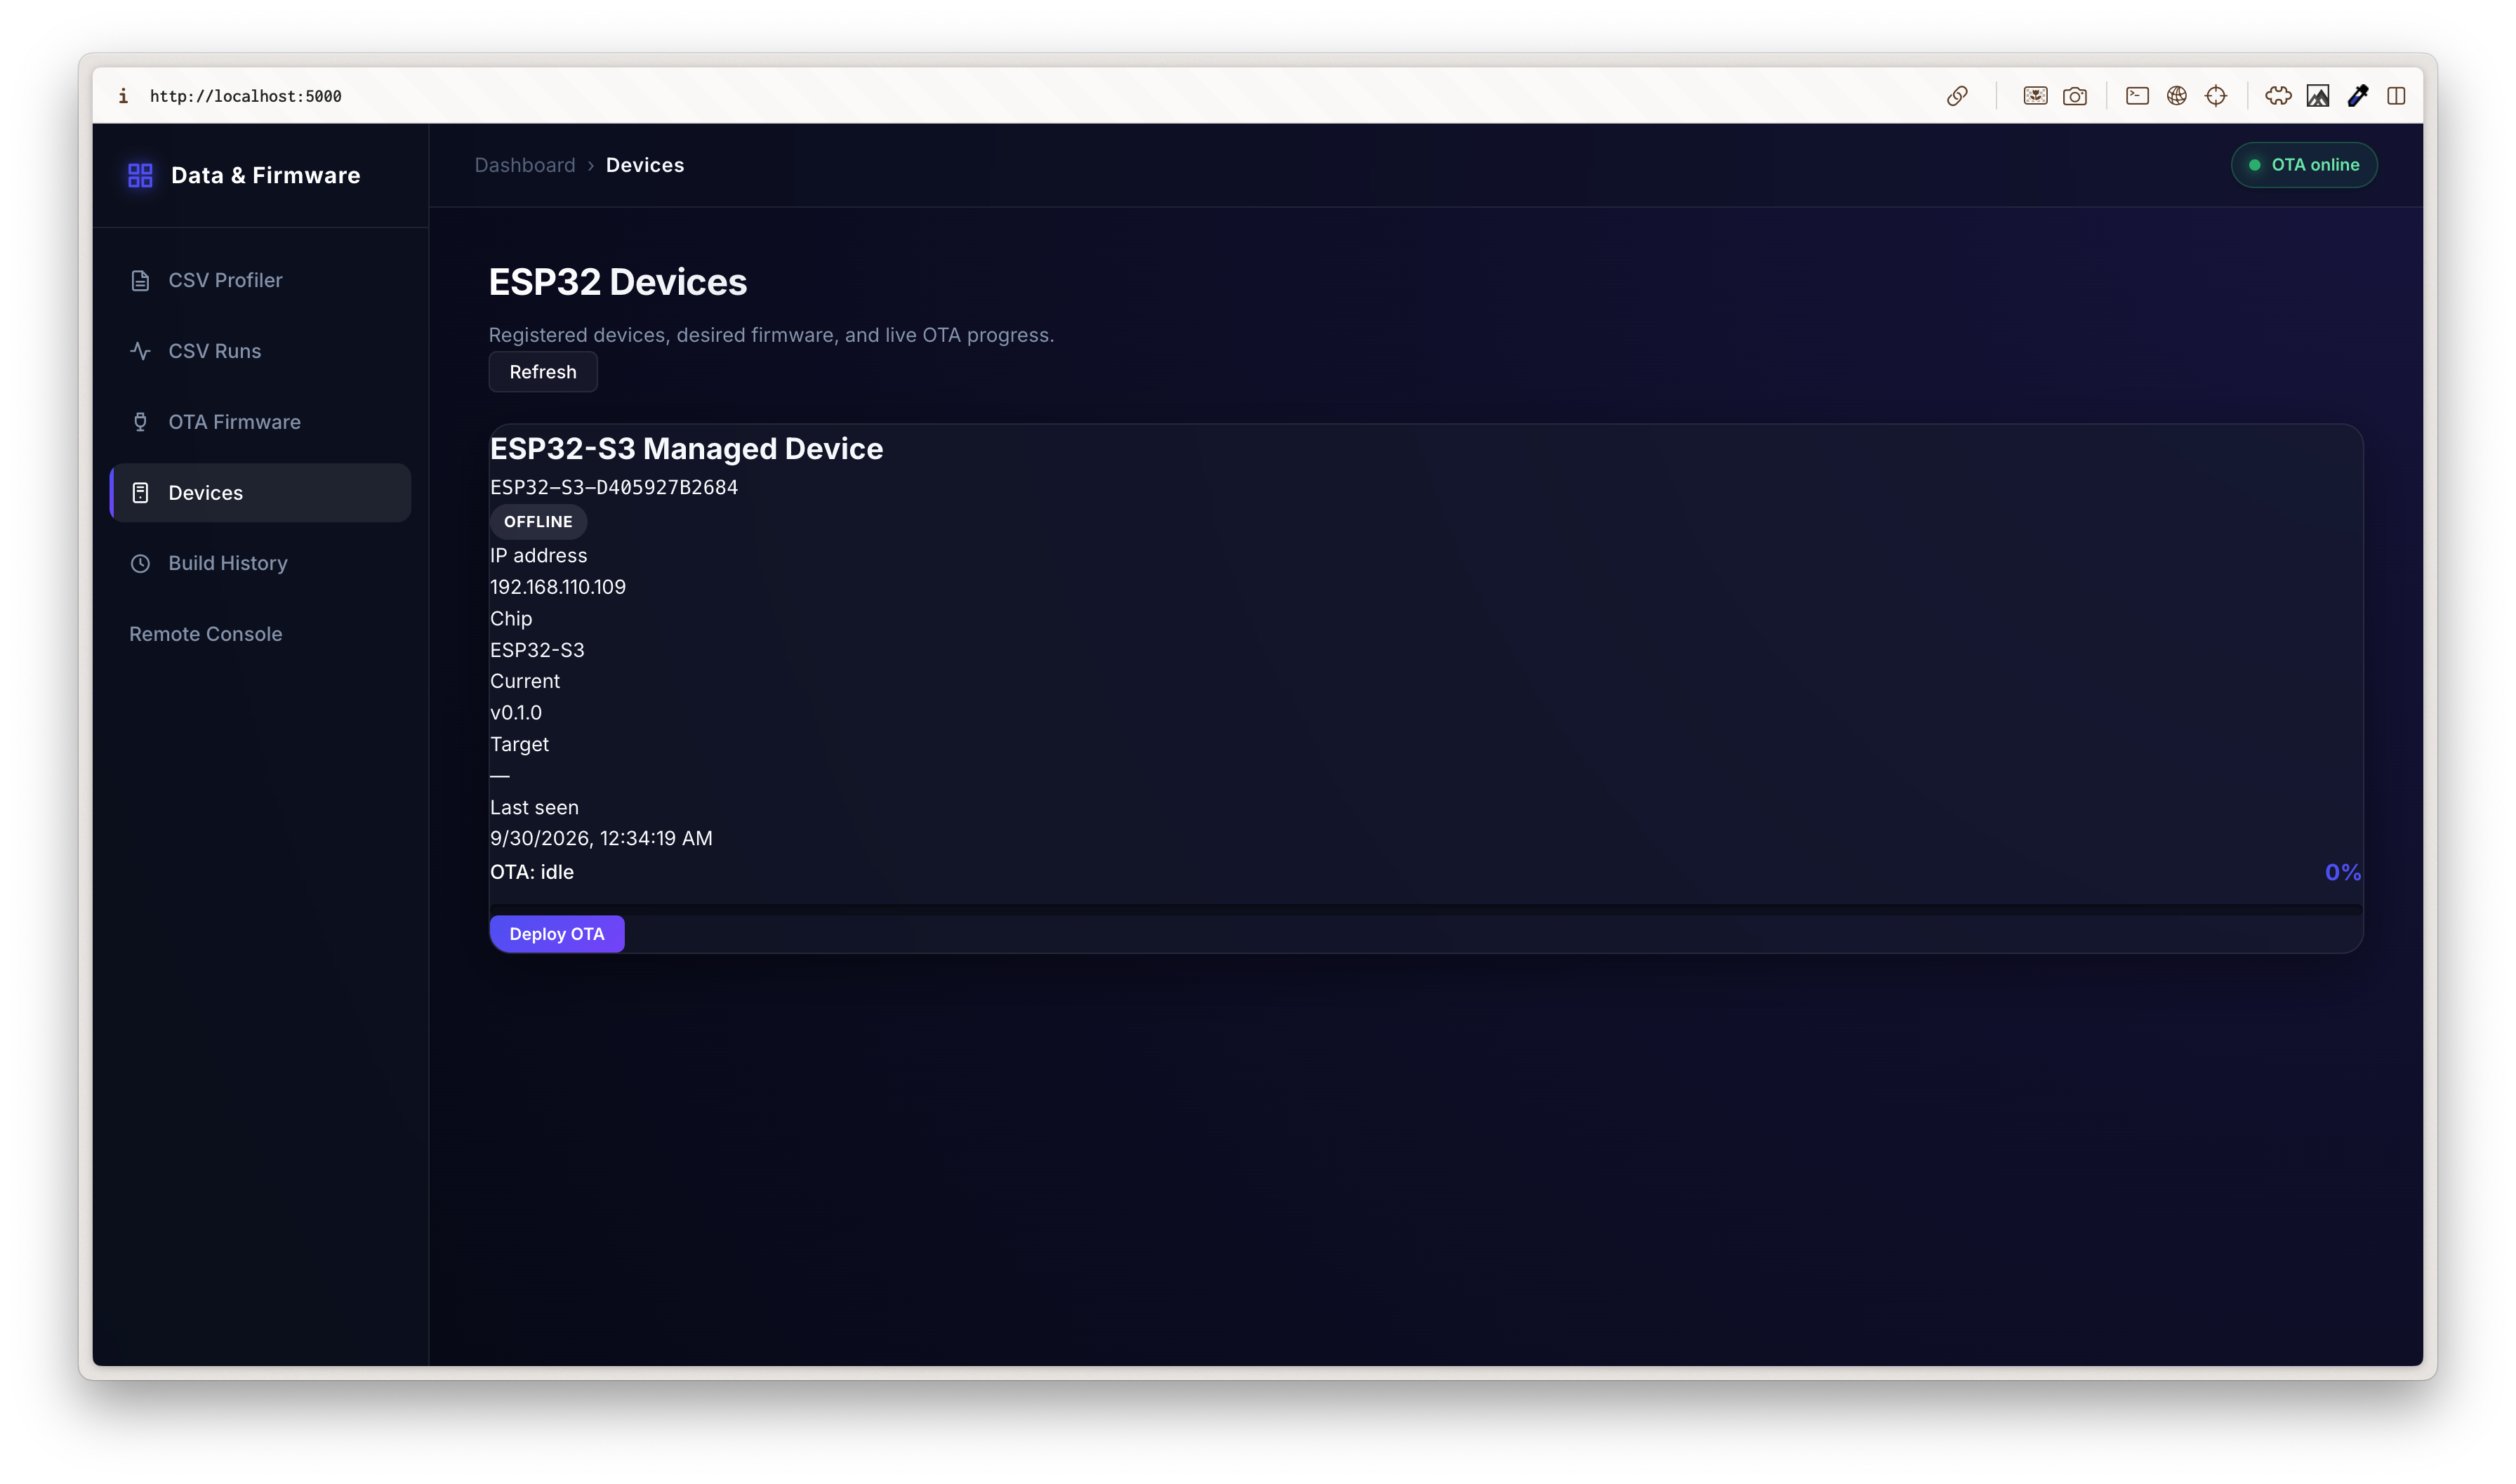
\includegraphics[width=0.88\textwidth]{ota_6.png}
  \caption{Halaman Devices --- ESP32-S3 terdaftar dengan status online.}
  \label{fig:devices}
\end{figure}

\begin{table}[H]
  \centering
  \caption{Informasi perangkat ESP32 terdaftar.}
  \label{tab:device_info}
  \begin{tabular}{ll}
    \toprule
    \textbf{Properti} & \textbf{Nilai} \\
    \midrule
    Device ID      & \texttt{ESP32-S3-D405927B2684} \\
    Chip           & ESP32-S3 \\
    IP Address     & 192.168.110.109 \\
    Versi Firmware & v0.1.0 \\
    Status OTA     & Idle \\
    \bottomrule
  \end{tabular}
\end{table}

\begin{figure}[H]
  \centering
  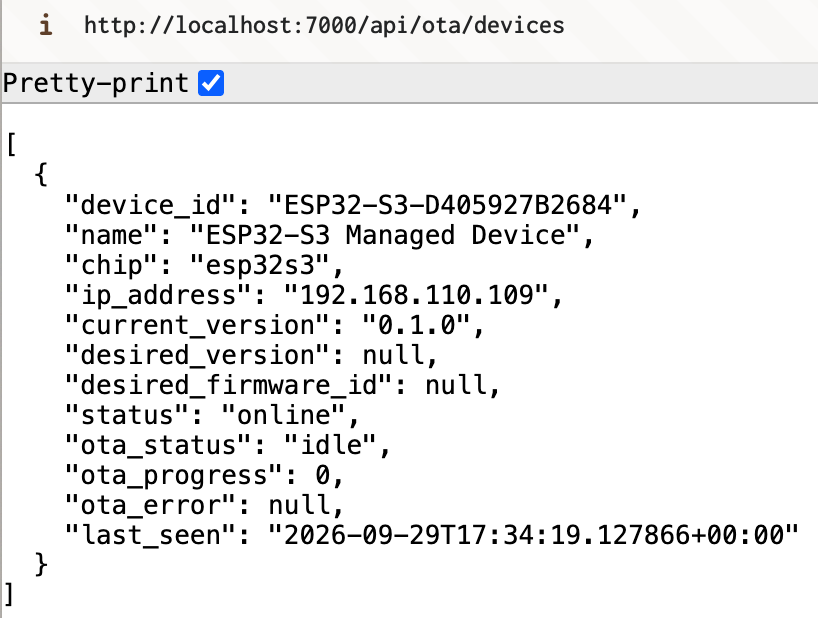
\includegraphics[width=0.72\textwidth]{ota_2.png}
  \caption{Respons REST API \texttt{GET /api/ota/devices}.}
  \label{fig:api_devices}
\end{figure}

\section{Halaman Build History}

\begin{figure}[H]
  \centering
  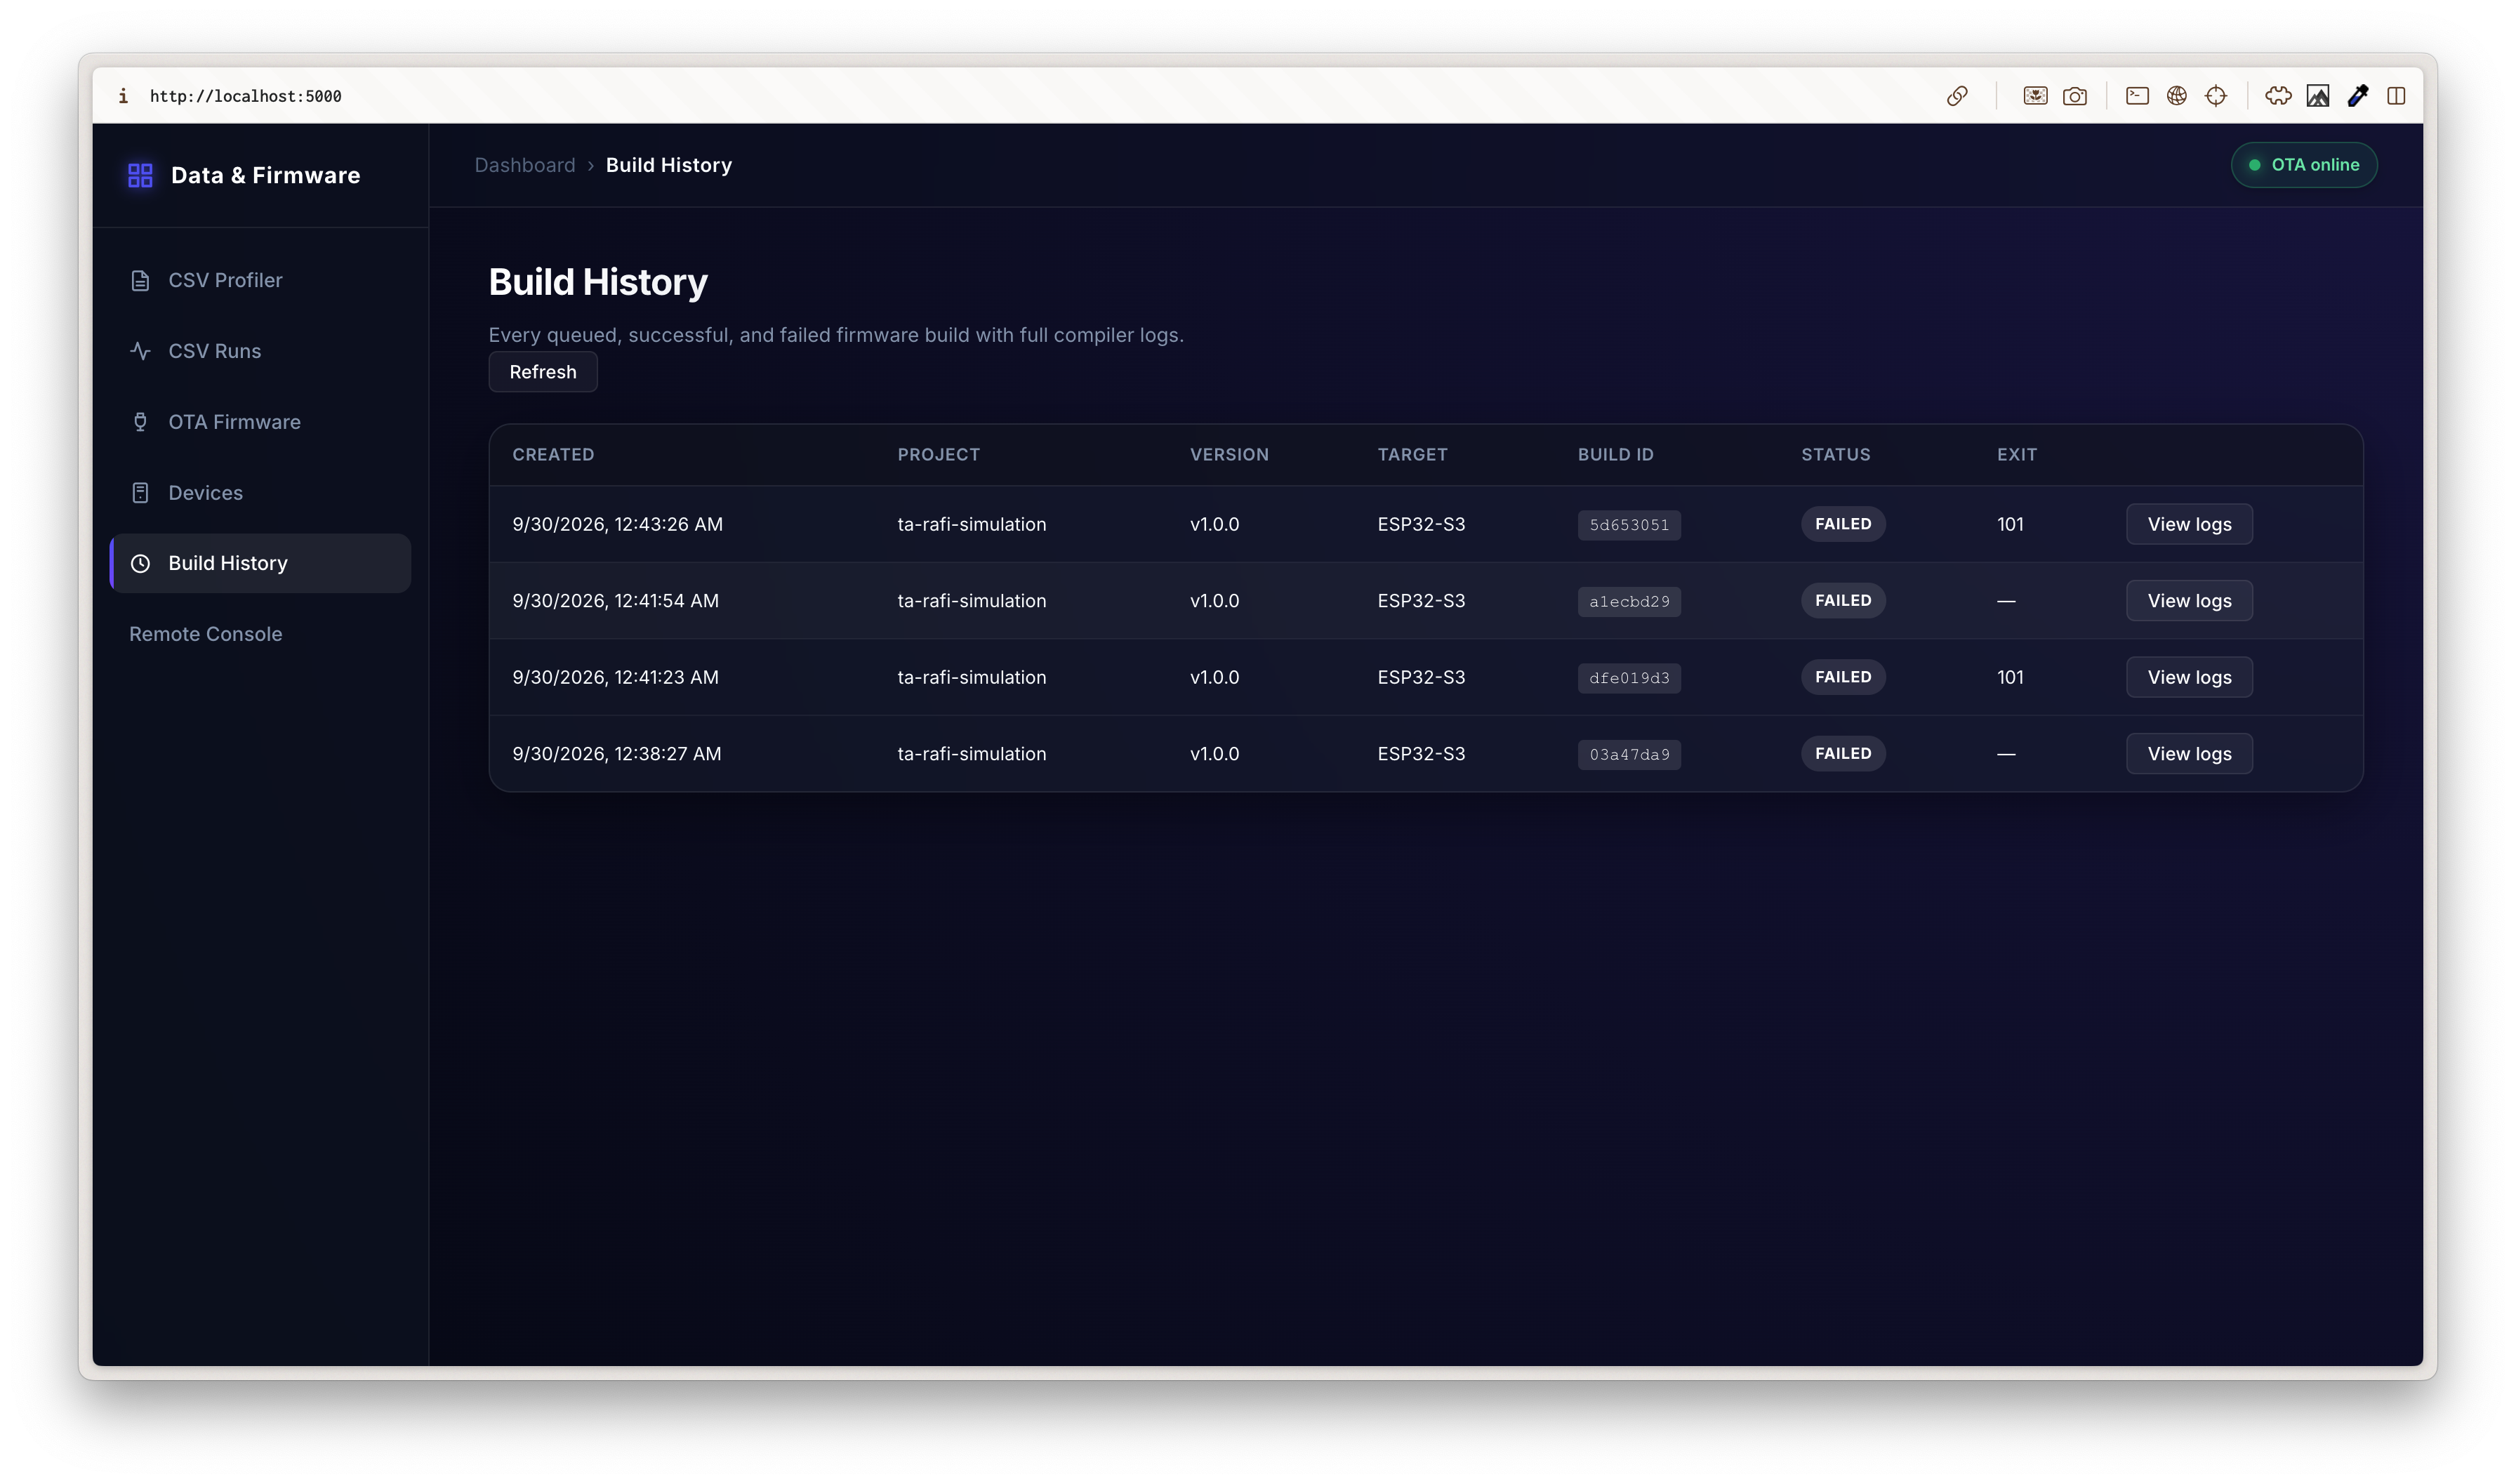
\includegraphics[width=0.88\textwidth]{ota_7.png}
  \caption{Build History --- riwayat build firmware proyek ESP32.}
  \label{fig:build_history}
\end{figure}

\begin{infobox}{Catatan Build}
  Build yang tercatat berstatus FAILED disebabkan oleh konfigurasi toolchain
  ESP-IDF yang belum lengkap. Ini kondisi yang diharapkan pada tahap awal.
\end{infobox}

\section{Remote Console}

\begin{figure}[H]
  \centering
  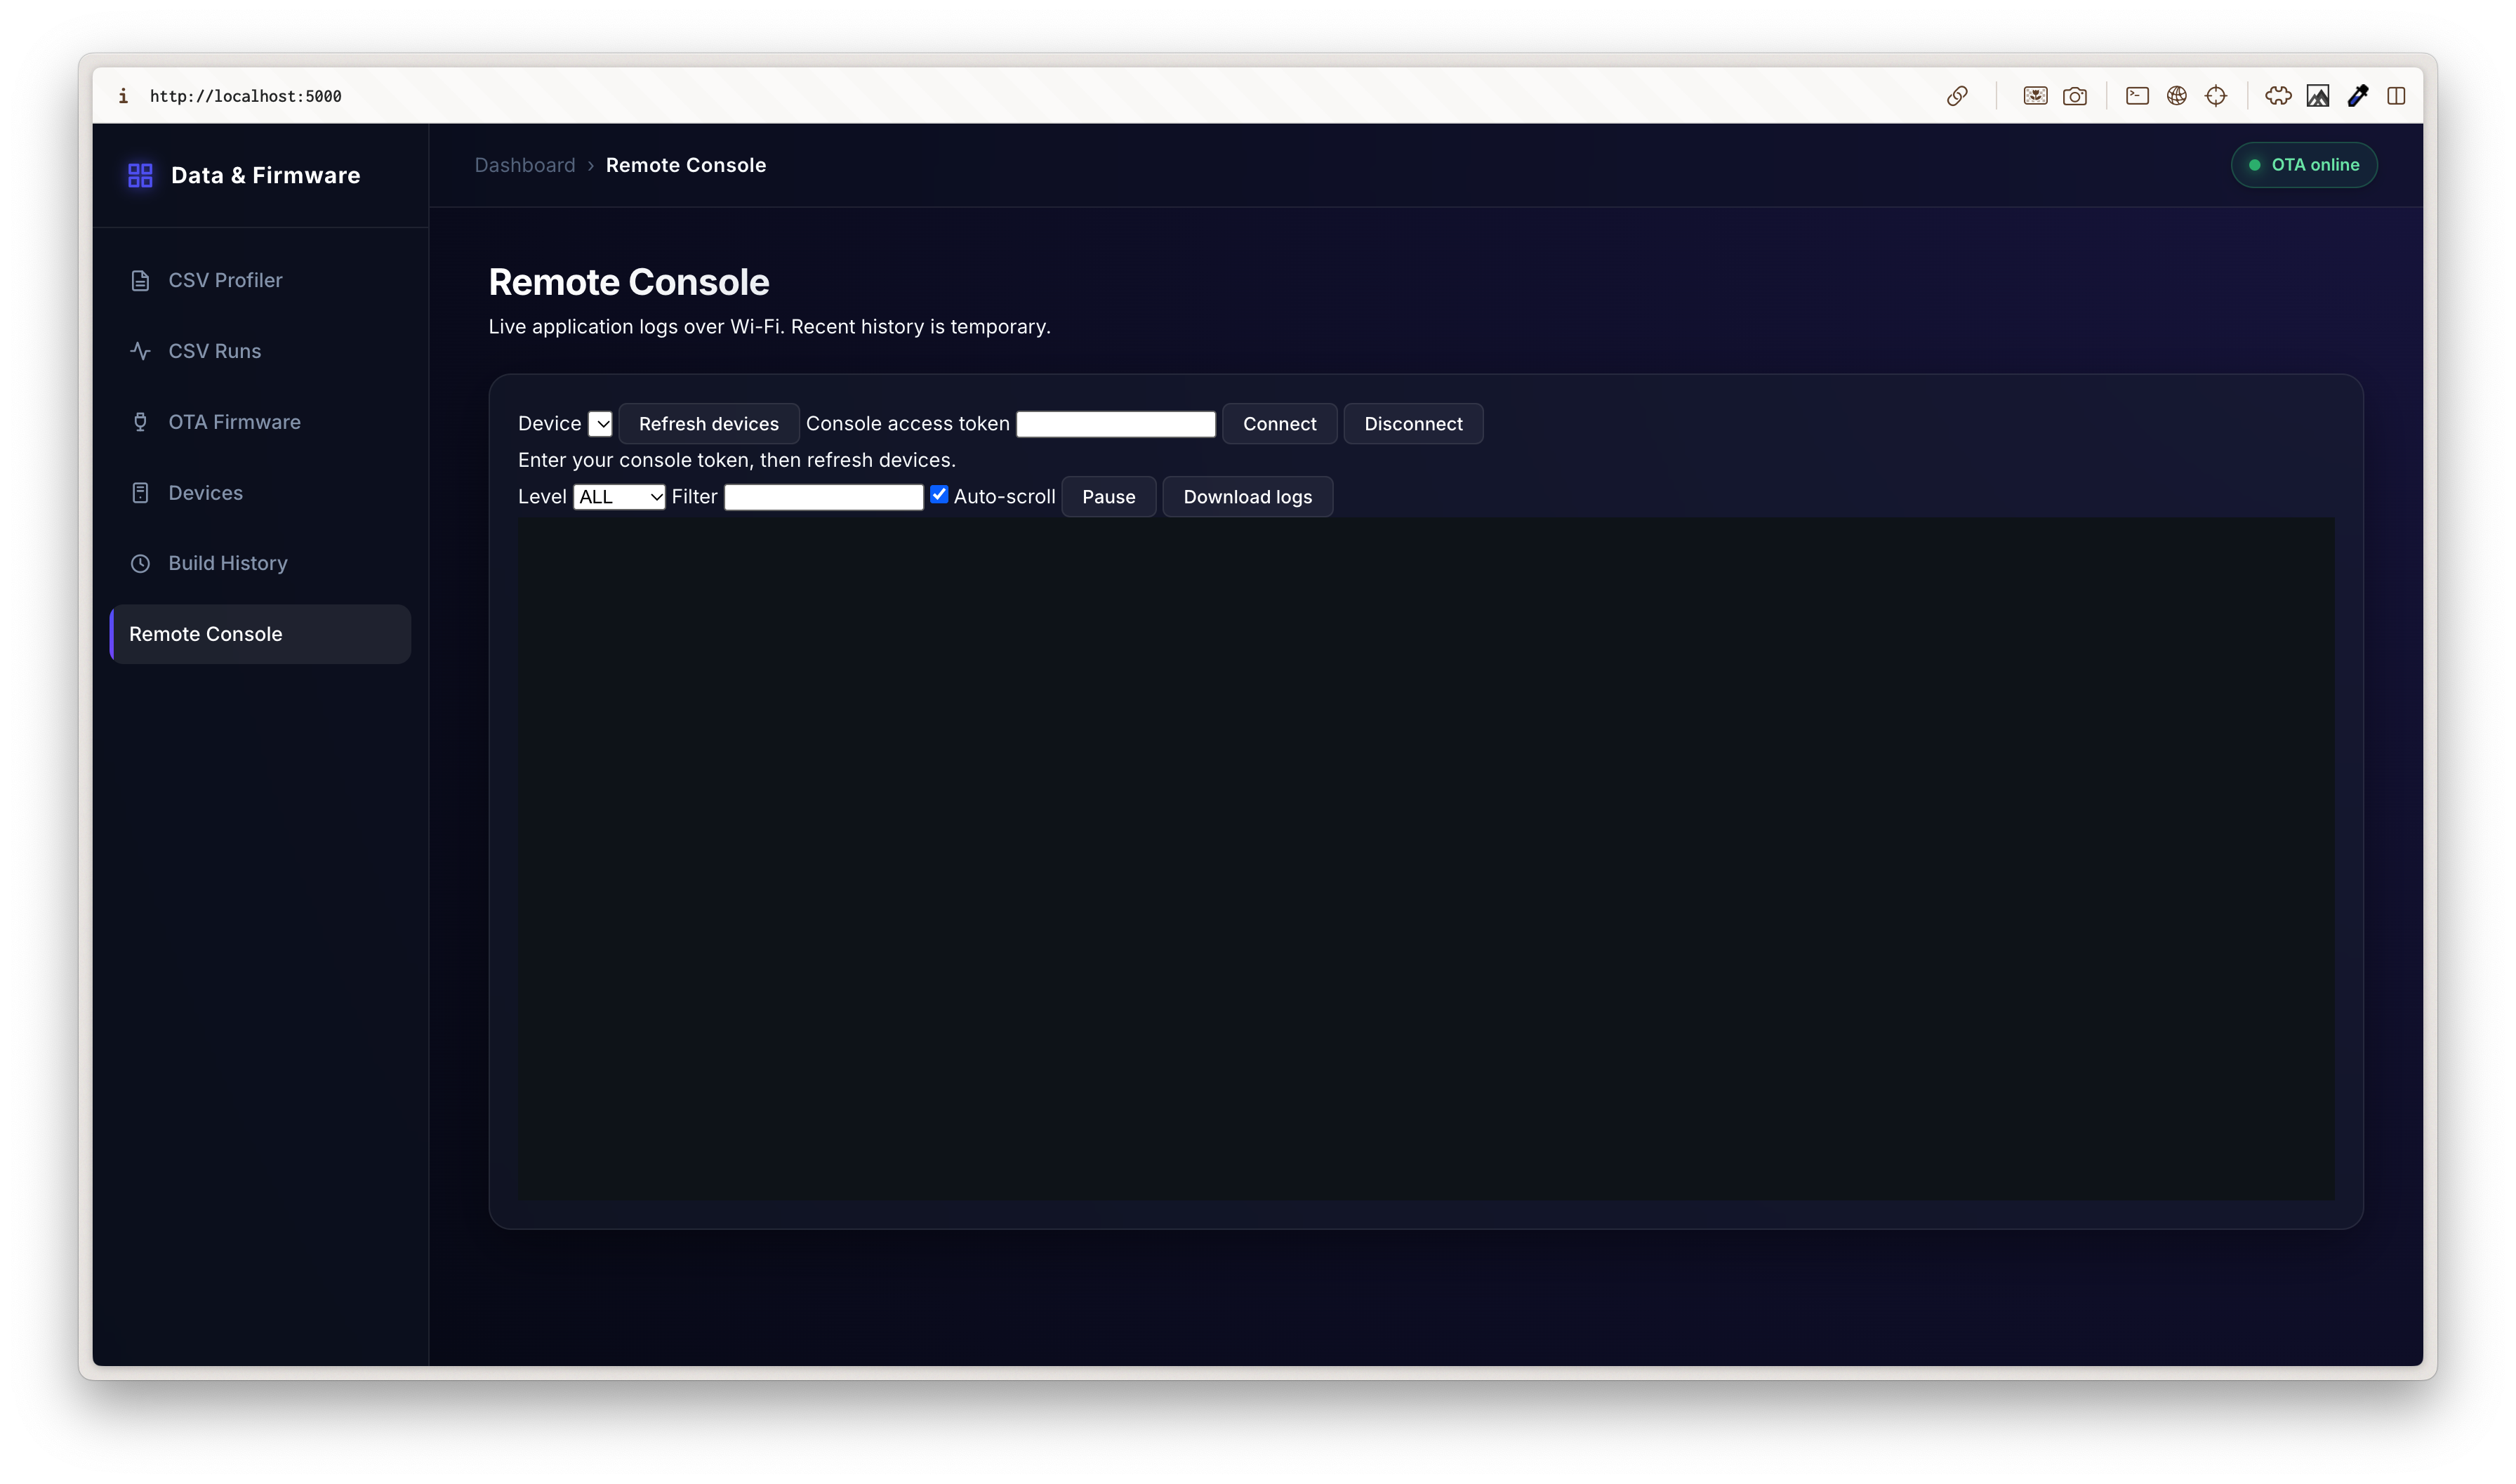
\includegraphics[width=0.88\textwidth]{ota_8.png}
  \caption{Remote Console --- monitoring log perangkat live via Wi-Fi.}
  \label{fig:remote_console}
\end{figure}

Fitur Remote Console memungkinkan pemantauan log aplikasi ESP32 secara
\textit{real-time} tanpa koneksi serial/USB, dengan filter level log dan
kemampuan download log untuk analisis offline.

%% ============================================================
\chapter{Firmware Simulasi ESP32 (Rust)}
%% ============================================================

\section{Gambaran Umum}

Firmware simulasi utama yang digunakan dalam sistem E-Nose ditulis menggunakan
bahasa \textbf{Rust} dan berjalan langsung di atas perangkat keras
\textbf{ESP32-S3} (\texttt{esp32\_simulation/src/main.rs}). Firmware ini
menggunakan ekosistem \texttt{esp-idf-hal} dan \texttt{esp-idf-svc} untuk
mengakses peripheral hardware secara aman.

Pendekatan ini dipilih karena:
\begin{itemize}[leftmargin=2cm, itemsep=2pt]
  \item \textbf{Tanpa sensor fisik}: Logika sensor disimulasikan secara
        matematis langsung di dalam firmware, sehingga tidak perlu ADC atau
        wiring sensor nyata selama pengembangan awal;
  \item \textbf{Dual connectivity}: Data dikirim secara bersamaan via
        \textbf{USB Serial UART} (untuk monitoring lokal) dan
        \textbf{ThingsBoard MQTT over WiFi} (untuk dashboard cloud);
  \item \textbf{Remote RPC}: Siklus pengujian dapat dikontrol
        (\texttt{START}/\texttt{STOP}) dari ThingsBoard Dashboard secara
        nirkabel melalui MQTT RPC;
  \item \textbf{Motor driver fisik}: Pin GPIO ESP32-S3 dikonfigurasi untuk
        mengontrol motor driver L298N (inlet/outlet) secara langsung.
\end{itemize}

\section{Arsitektur Koneksi}

\begin{table}[H]
  \centering
  \caption{Konfigurasi koneksi firmware simulasi ESP32.}
  \label{tab:koneksi_fw}
  \begin{tabularx}{\textwidth}{>{\bfseries}p{3.6cm} p{4.6cm} X}
    \toprule
    \textbf{Jalur} & \textbf{Protokol} & \textbf{Fungsi} \\
    \midrule
    USB Serial UART       & UART0 / stdout                                                           & Output JSON telemetri lokal \\
    WiFi + MQTT           & TCP port 1883                                                            & Kirim telemetri ke ThingsBoard Cloud \\
    MQTT RPC Subscribe    & Topic: \newline \texttt{v1/devices/me/}\allowbreak\texttt{rpc/request/+} & Terima perintah START/STOP dari dashboard \\
    Driver Motor A (GPIO) & Digital OUT                                                              & Inlet pump \& valve (pin 5, 17, 14, 19) \\
    Driver Motor B (GPIO) & Digital OUT                                                              & Outlet pump \& valve (pin 16, 4, 45, 20) \\
    \bottomrule
  \end{tabularx}
\end{table}

\section{Arsitektur Siklus Pengujian Tiga Fase}

Setiap siklus pengujian berlangsung \textbf{300 detik} dalam tiga fase yang
dikontrol secara otomatis oleh firmware:

\begin{table}[H]
  \centering
  \caption{Tiga fase siklus pengujian E-Nose dalam firmware Rust.}
  \label{tab:fases}
  \begin{tabular}{clll}
    \toprule
    \textbf{Fase} & \textbf{Waktu} & \textbf{Motor Driver} & \textbf{Respons Sensor} \\
    \midrule
    1 & 1 -- 70 detik    & Driver A \& B OFF (Purge) & Baseline \\
    2 & 71 -- 170 detik  & Driver A ON (Inlet)        & Naik eksponensial \\
    3 & 171 -- 300 detik & Driver B ON (Outlet)       & Turun eksponensial \\
    \bottomrule
  \end{tabular}
\end{table}

\subsection{Model Matematika Respons Sensor}

Model sensor diimplementasikan sebagai fungsi \texttt{simulate\_sensors()} dalam
Rust. Faktor respons dihitung berdasarkan fase aktif:

\begin{itemize}[leftmargin=2cm]
  \item \textbf{Fase Inlet (kenaikan eksponensial):}
        \[
          f_{\text{naik}}(t) = 1 - e^{-2.6 \cdot \frac{t - 70}{100}}
        \]
  \item \textbf{Fase Outlet (penurunan eksponensial):}
        \[
          f_{\text{turun}}(t) = e^{-3.2 \cdot \frac{t - 170}{130}}
        \]
  \item \textbf{Nilai tegangan sensor akhir:}
        \[
          V_{\text{sensor}} = V_{\text{baseline}}
            + (V_{\text{peak}} - V_{\text{baseline}}) \cdot f
            + \varepsilon, \quad \varepsilon \sim \mathcal{U}(-12,+12)\,\text{mV}
        \]
\end{itemize}

Noise sensor $\varepsilon$ dibangkitkan menggunakan Linear Congruential Generator
(LCG) bawaan tanpa library tambahan, agar firmware tetap minimalis.

\subsection{Parameter Sensor}

\begin{table}[H]
  \centering
  \caption{Parameter baseline dan peak voltage delapan sensor gas (mV).}
  \label{tab:sensor_params}
  \begin{tabular}{lcc}
    \toprule
    \textbf{Sensor} & \textbf{Baseline (mV)} & \textbf{Peak (mV)} \\
    \midrule
    MQ-6    & 460  & 1850 \\
    MQ-135  & 530  & 2400 \\
    MQ-3    & 390  & 2950 \\
    MQ-7    & 610  & 1780 \\
    TGS2611 & 430  & 2380 \\
    TGS2602 & 560  & 2820 \\
    TGS2600 & 400  & 2120 \\
    TGS2620 & 490  & 2640 \\
    \bottomrule
  \end{tabular}
\end{table}

\section{Cuplikan Kode Firmware Rust}

\subsection{Fungsi Simulasi Sensor}

\begin{lstlisting}[language={[ANSI]C},
    caption={Fungsi \texttt{simulate\_sensors()} --- kalkulasi respons sensor
             per fase dalam Rust (esp32\_simulation/src/main.rs).}]
fn simulate_sensors(state: &mut SystemState, seed: &mut u32) {
    let elapsed = get_elapsed_time(state);

    let factor = if !state.running || elapsed <= 70 {
        0.0f32  // Fase 1: Standby / Baseline
    } else if elapsed <= 170 {
        // Fase 2: Inlet ON - kurva naik eksponensial
        let progress = (elapsed - 70) as f32 / 100.0;
        1.0 - (-2.6 * progress).exp()
    } else if elapsed <= 300 {
        // Fase 3: Outlet ON - kurva turun eksponensial
        let progress = (elapsed - 170) as f32 / 130.0;
        (-3.2 * progress).exp()
    } else {
        0.0f32
    };

    let noise = |s: &mut u32| rand_range(s, -12.0, 12.0);
    state.sensors.mq6 =
        (460.0 + (1850.0 - 460.0) * factor + noise(seed)).max(50.0);
    state.sensors.mq135 =
        (530.0 + (2400.0 - 530.0) * factor + noise(seed)).max(50.0);
    // ... (sensor lainnya dengan pola yang sama)
    state.sensors.dht_temp = 27.5 + rand_range(seed, -0.2, 0.2);
    state.sensors.dht_hum  = 62.0 + rand_range(seed, -0.8, 0.8);
}
\end{lstlisting}

\subsection{Pengiriman Telemetri ke ThingsBoard via MQTT}

\begin{lstlisting}[language={[ANSI]C},
    caption={Fungsi \texttt{send\_thingsboard\_telemetry()} --- publish MQTT ke
             ThingsBoard Cloud tiap 1 detik.}]
fn send_thingsboard_telemetry(
    state: &SystemState,
    mqtt: &mut Option<EspMqttClient>
) {
    if let Some(client) = mqtt {
        let payload = format!(
            "{\"mq6\":{:.2}, \"mq135\":{:.2}, ...,
             \"inlet_pump\":{}, \"outlet_pump\":{},
             \"elapsed_time\":{}, \"running\":{}}",
            s.mq6, s.mq135, /* ... */
            state.driver1_active, state.driver2_active,
            get_elapsed_time(state), state.running,
        );
        client.publish(
            "v1/devices/me/telemetry",
            QoS::AtLeastOnce,
            false,
            payload.as_bytes(),
        ).ok();
    }
}
\end{lstlisting}

\subsection{Remote RPC Control dari ThingsBoard}

Firmware berlangganan (\textit{subscribe}) ke topic MQTT RPC ThingsBoard
untuk menerima perintah \texttt{START} / \texttt{STOP} dari dashboard:

\begin{lstlisting}[language={[ANSI]C},
    caption={Handler MQTT RPC --- menerima perintah START/STOP dari
             ThingsBoard Dashboard secara nirkabel.}]
EventPayload::Received { topic, data, .. } => {
    if let Some(t) = topic {
        if t.starts_with("v1/devices/me/rpc/request/") {
            let req_id = &t["v1/devices/me/rpc/request/".len()..];
            let upper = payload_str.to_uppercase();
            if upper.contains("START") {
                rpc_cmd_queue.lock().unwrap().push("START".to_string());
            } else if upper.contains("STOP") {
                rpc_cmd_queue.lock().unwrap().push("STOP".to_string());
            }
            // Kirim balasan RPC
            let resp_topic = format!("v1/devices/me/rpc/response/{}", req_id);
            client.publish(&resp_topic, QoS::AtLeastOnce, false,
                           b"{\"status\":\"ok\"}");
        }
    }
}
\end{lstlisting}

\subsection{Visualisasi Telemetri pada ThingsBoard Cloud}

Data telemetri yang dikirimkan oleh firmware ESP32-S3 diterima dan divisualisasikan
secara \textit{real-time} pada antarmuka ThingsBoard Cloud sebagaimana ditunjukkan pada
Gambar~\ref{fig:thingsboard_dashboard}.

\begin{figure}[H]
  \centering
  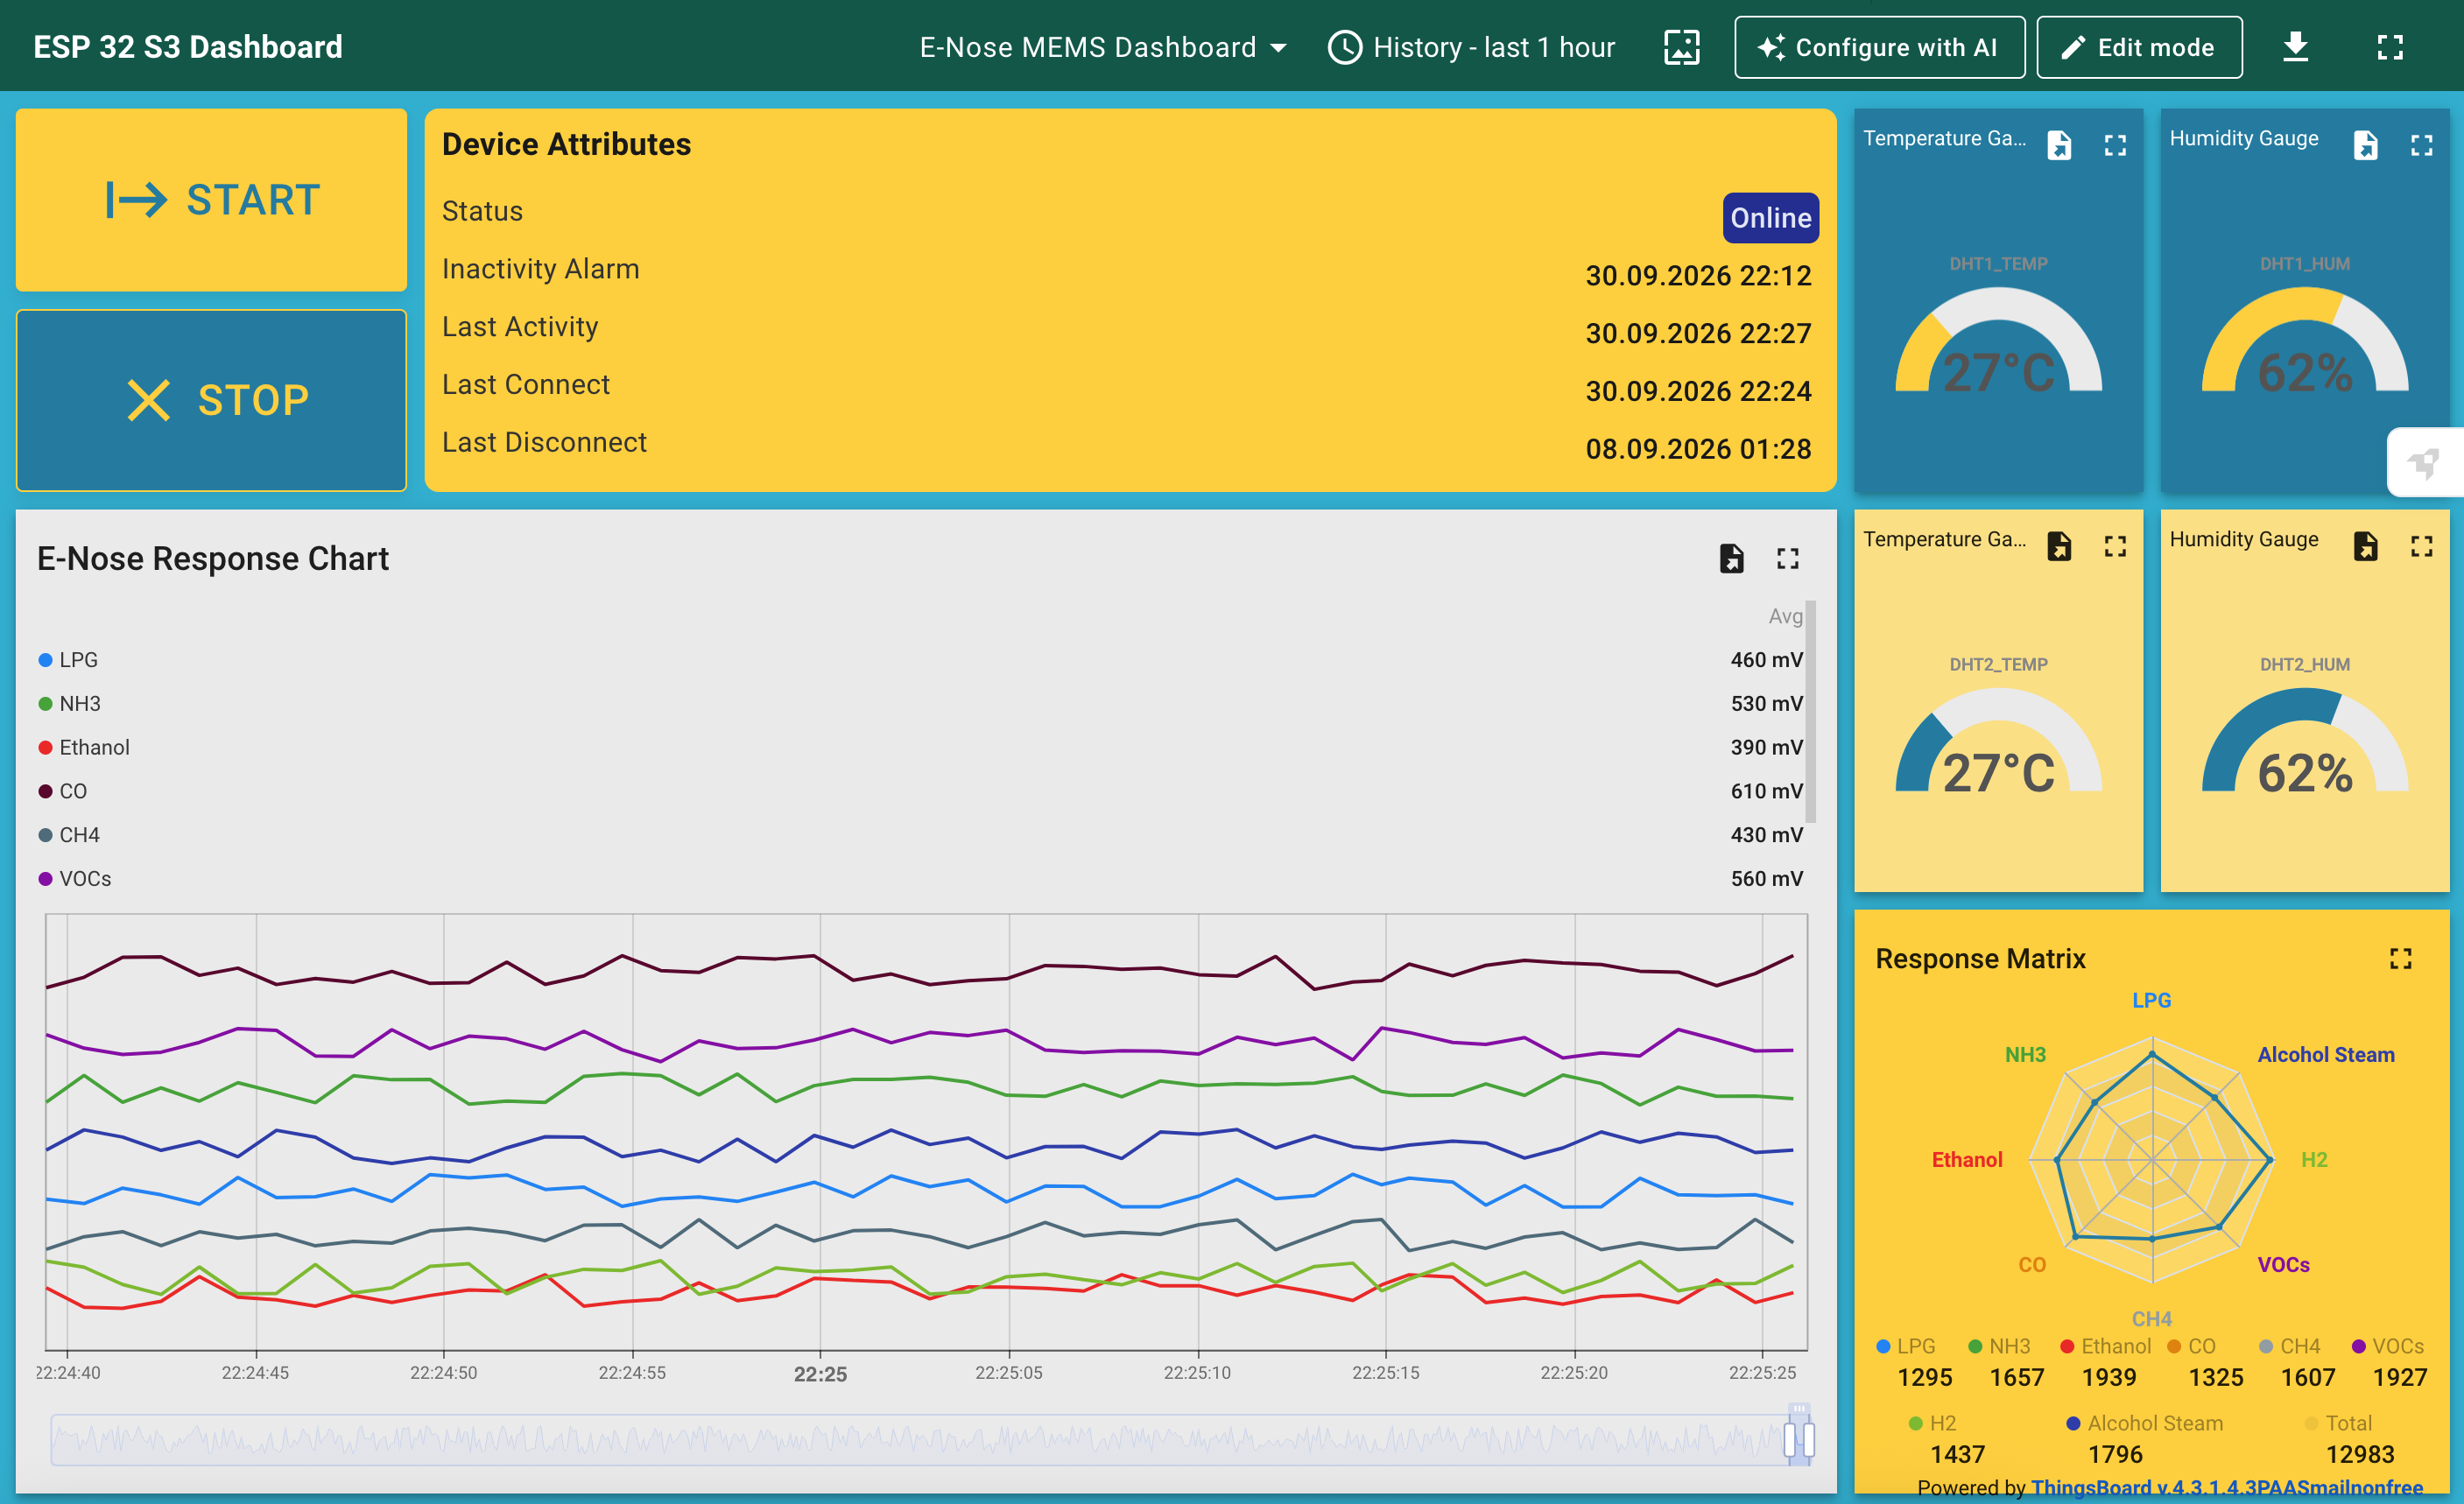
\includegraphics[width=0.95\textwidth]{thingsboard.png}
  \caption{Dashboard E-Nose pada ThingsBoard Cloud --- grafik respons multi-sensor (LPG, NH3, Ethanol, CO, CH4, VOCs), matriks respons radar, indikator suhu/kelembaban DHT22, status koneksi perangkat (Online), serta tombol kontrol RPC (\texttt{START} dan \texttt{STOP}).}
  \label{fig:thingsboard_dashboard}
\end{figure}

Dashboard ini menyediakan:
\begin{itemize}[leftmargin=2cm, itemsep=2pt]
  \item \textbf{E-Nose Response Chart}: Grafik kurva dinamis yang memperlihatkan nilai tegangan (mV) masing-masing sensor gas secara kontinu;
  \item \textbf{Response Matrix (Radar Chart)}: Pemetaan sebaran sensitivitas antar gas secara simultan untuk identifikasi profil aroma;
  \item \textbf{Environmental Gauges}: Pemantauan kondisi lingkungan (suhu dan kelembaban relatif) dari sensor DHT22;
  \item \textbf{Device Attributes \& RPC Control}: Indikator status perangkat (\textit{Online}) dan tombol interaktif untuk memulai (\texttt{START}) atau menghentikan (\texttt{STOP}) siklus pengujian dari jarak jauh.
\end{itemize}

\section{Output JSON via UART Serial}

Selain ThingsBoard, setiap pembacaan sensor juga dikirim melalui USB Serial
dalam format JSON terstruktur. Hal ini memudahkan monitoring langsung dari
terminal komputer saat debugging:

\begin{lstlisting}[language=bash,
    caption={Contoh output JSON dari UART Serial ESP32 tiap 1 detik.}]
{
  "sensors": {
    "mq6": 1234.56, "mq135": 1876.32, "mq3": 2501.10,
    "mq7": 1102.45, "tgs2611": 1650.00, "tgs2602": 1890.70,
    "tgs2600": 1550.22, "tgs2620": 1750.80,
    "dht_temp": 27.48, "dht_hum": 62.13
  },
  "status": {
    "inlet_pump": true, "inlet_valve": true,
    "outlet_pump": false, "outlet_valve": false,
    "inlet_time": 45, "outlet_time": 0, "elapsed_time": 115
  },
  "timestamp": 115432
}
\end{lstlisting}

\section{Cara Build, Flash, dan Hasil Eksekusi}

Firmware di-build menggunakan toolchain Rust untuk ESP32 (esp-rs) dan
di-flash menggunakan \texttt{cargo espflash} dengan menyertakan tabel partisi kustom:

\begin{lstlisting}[language=bash,
    caption={Perintah build dan flash firmware simulasi ke ESP32-S3.}]
cd esp32_simulation
cargo build --release
cargo espflash flash --release --partition-table partitions.csv --monitor
\end{lstlisting}

Setelah proses flashing selesai, Serial Monitor pada terminal komputer menampilkan
log proses inisialisasi jaringan Wi-Fi, koneksi ke MQTT broker ThingsBoard Cloud,
serta aliran telemetri JSON yang berhasil dikirimkan setiap detik (Gambar~\ref{fig:esp_log}).

\begin{figure}[H]
  \centering
  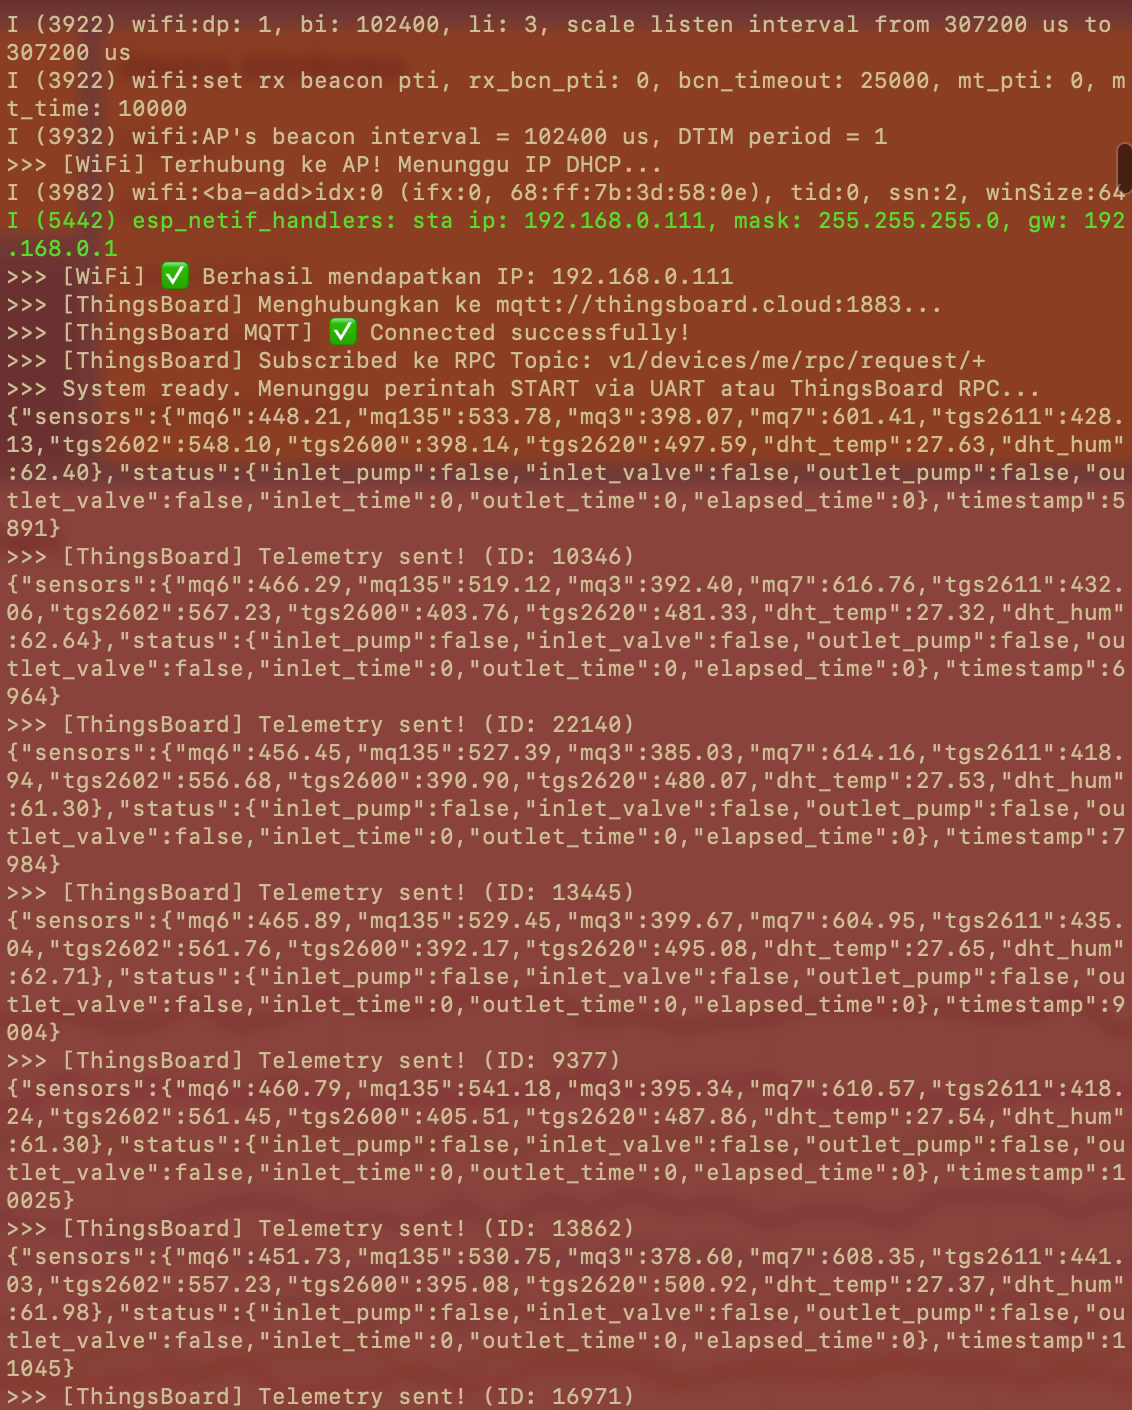
\includegraphics[width=0.80\textwidth]{esp_log.png}
  \caption{Log terminal Serial Monitor ESP32-S3 --- verifikasi koneksi Wi-Fi berhasil mendapatkan IP DHCP, terhubung ke ThingsBoard MQTT, dan pengiriman stream telemetri JSON secara real-time.}
  \label{fig:esp_log}
\end{figure}

%% ============================================================
\chapter{Lingkungan Pengembangan}
%% ============================================================

\section{Spesifikasi Mesin Pengembangan}

\begin{table}[H]
  \centering
  \caption{Spesifikasi mesin pengembangan.}
  \label{tab:mesin}
  \begin{tabular}{ll}
    \toprule
    \textbf{Komponen} & \textbf{Spesifikasi} \\
    \midrule
    Sistem Operasi  & macOS \\
    Python          & 3.x (virtual environment \texttt{uv}) \\
    Rust / Cargo    & Stable channel \\
    Paket Python    & Flask, ydata-profiling, pandas, numpy \\
    \bottomrule
  \end{tabular}
\end{table}

\section{Struktur Direktori Proyek}

\begin{lstlisting}[language=bash, caption={Struktur direktori proyek E-Nose.}]
TA-Rafi-Cepmek/
|-- CSV_PROFILING-main/      # Dashboard CSV Profiler + OTA Server
|   |-- python/              # Flask backend (profiler_server.py)
|   |-- src/                 # Rust backend (Axum OTA Server)
|   |-- static/              # Frontend web (HTML/CSS/JS)
|   |-- run-dev.sh           # Script untuk menjalankan semua server
|   +-- .env                 # Konfigurasi environment
|-- esp32_simulation/        # Firmware simulasi sensor E-Nose
|   |-- src/
|   |   +-- main.rs          # Firmware Rust (ESP32-S3, WiFi, MQTT, GPIO)
|   |-- Cargo.toml           # Rust project manifest
|   +-- sdkconfig.defaults   # Konfigurasi ESP-IDF
+-- docs/
    +-- image/               # Screenshot dan gambar dokumentasi
\end{lstlisting}

\section{Kendala Teknis dan Solusi}

\begin{table}[H]
  \centering
  \caption{Kendala teknis dan solusi yang diterapkan.}
  \label{tab:kendala}
  \begin{tabular}{p{0.38\textwidth}p{0.52\textwidth}}
    \toprule
    \textbf{Kendala} & \textbf{Solusi} \\
    \midrule
    \texttt{ModuleNotFoundError: flask} &
    Membuat ulang \texttt{venv} dengan \texttt{uv} pada macOS
    (venv lama dibuat di Windows). \\[6pt]
    \texttt{Address already in use (port 7000)} &
    \texttt{lsof -ti :7000 | xargs kill -9} \\[6pt]
    Deprecation \texttt{ydata\_profiling} &
    Dicatat sebagai technical debt; fungsionalitas normal.
    Migrasi ke \texttt{fg-data-profiling} direncanakan. \\
    \bottomrule
  \end{tabular}
\end{table}

%% ============================================================
\chapter{Kesimpulan dan Rencana Selanjutnya}
%% ============================================================

\section{Kesimpulan Progress}

Pada tahap ini, telah berhasil dikembangkan dan diuji tiga komponen infrastruktur:

\begin{enumerate}[leftmargin=2cm, itemsep=4pt]
  \item \textbf{CSV Data Profiler} --- menghasilkan laporan EDA otomatis lengkap
        termasuk statistik deskriptif, analisis korelasi, dan visualisasi sensor.

  \item \textbf{OTA Firmware Server} --- menyediakan semua fitur manajemen
        firmware: upload/build, manajemen perangkat, riwayat build, dan remote console.

  \item \textbf{Simulasi Telemetri} --- berhasil mensimulasikan siklus 3 fase dan
        mengirimkan data ke ThingsBoard Cloud secara real-time.
\end{enumerate}

\section{Rencana Tahap Selanjutnya}

\begin{table}[H]
  \centering
  \caption{Rencana kerja tahap berikutnya.}
  \label{tab:rencana}
  \begin{tabular}{clc}
    \toprule
    \textbf{No.} & \textbf{Rencana Kerja} & \textbf{Status} \\
    \midrule
    1 & Pengujian dan validasi flashing firmware ke ESP32 & Belum dimulai \\
    2 & Integrasi modul klien OTA pada firmware ESP32     & Belum dimulai \\
    3 & Pengujian OTA update nirkabel via OTA Server      & Belum dimulai \\
    4 & Implementasi algoritma klasifikasi aroma gas (ML) & Belum dimulai \\
    5 & Migrasi ke \texttt{fg-data-profiling}             & Direncanakan \\
    \bottomrule
  \end{tabular}
\end{table}

\vspace{1cm}
\hrule
\vspace{0.5cm}
{\small\textit{Laporan ini dibuat pada \today\ sebagai dokumentasi progress
Tugas Akhir. Seluruh kode dan tangkapan layar merupakan hasil kerja nyata
pada lingkungan pengembangan penulis.}}

\end{document}
